% Options for packages loaded elsewhere
\PassOptionsToPackage{unicode}{hyperref}
\PassOptionsToPackage{hyphens}{url}
%
\documentclass[
]{book}
\usepackage{amsmath,amssymb}
\usepackage{lmodern}
\usepackage{iftex}
\ifPDFTeX
  \usepackage[T1]{fontenc}
  \usepackage[utf8]{inputenc}
  \usepackage{textcomp} % provide euro and other symbols
\else % if luatex or xetex
  \usepackage{unicode-math}
  \defaultfontfeatures{Scale=MatchLowercase}
  \defaultfontfeatures[\rmfamily]{Ligatures=TeX,Scale=1}
\fi
% Use upquote if available, for straight quotes in verbatim environments
\IfFileExists{upquote.sty}{\usepackage{upquote}}{}
\IfFileExists{microtype.sty}{% use microtype if available
  \usepackage[]{microtype}
  \UseMicrotypeSet[protrusion]{basicmath} % disable protrusion for tt fonts
}{}
\makeatletter
\@ifundefined{KOMAClassName}{% if non-KOMA class
  \IfFileExists{parskip.sty}{%
    \usepackage{parskip}
  }{% else
    \setlength{\parindent}{0pt}
    \setlength{\parskip}{6pt plus 2pt minus 1pt}}
}{% if KOMA class
  \KOMAoptions{parskip=half}}
\makeatother
\usepackage{xcolor}
\IfFileExists{xurl.sty}{\usepackage{xurl}}{} % add URL line breaks if available
\IfFileExists{bookmark.sty}{\usepackage{bookmark}}{\usepackage{hyperref}}
\hypersetup{
  pdftitle={SCMA470 Risk Analysis and Credibility},
  pdfauthor={Pairote Satiracoo},
  hidelinks,
  pdfcreator={LaTeX via pandoc}}
\urlstyle{same} % disable monospaced font for URLs
\usepackage[margin=1in]{geometry}
\usepackage{color}
\usepackage{fancyvrb}
\newcommand{\VerbBar}{|}
\newcommand{\VERB}{\Verb[commandchars=\\\{\}]}
\DefineVerbatimEnvironment{Highlighting}{Verbatim}{commandchars=\\\{\}}
% Add ',fontsize=\small' for more characters per line
\usepackage{framed}
\definecolor{shadecolor}{RGB}{248,248,248}
\newenvironment{Shaded}{\begin{snugshade}}{\end{snugshade}}
\newcommand{\AlertTok}[1]{\textcolor[rgb]{0.94,0.16,0.16}{#1}}
\newcommand{\AnnotationTok}[1]{\textcolor[rgb]{0.56,0.35,0.01}{\textbf{\textit{#1}}}}
\newcommand{\AttributeTok}[1]{\textcolor[rgb]{0.77,0.63,0.00}{#1}}
\newcommand{\BaseNTok}[1]{\textcolor[rgb]{0.00,0.00,0.81}{#1}}
\newcommand{\BuiltInTok}[1]{#1}
\newcommand{\CharTok}[1]{\textcolor[rgb]{0.31,0.60,0.02}{#1}}
\newcommand{\CommentTok}[1]{\textcolor[rgb]{0.56,0.35,0.01}{\textit{#1}}}
\newcommand{\CommentVarTok}[1]{\textcolor[rgb]{0.56,0.35,0.01}{\textbf{\textit{#1}}}}
\newcommand{\ConstantTok}[1]{\textcolor[rgb]{0.00,0.00,0.00}{#1}}
\newcommand{\ControlFlowTok}[1]{\textcolor[rgb]{0.13,0.29,0.53}{\textbf{#1}}}
\newcommand{\DataTypeTok}[1]{\textcolor[rgb]{0.13,0.29,0.53}{#1}}
\newcommand{\DecValTok}[1]{\textcolor[rgb]{0.00,0.00,0.81}{#1}}
\newcommand{\DocumentationTok}[1]{\textcolor[rgb]{0.56,0.35,0.01}{\textbf{\textit{#1}}}}
\newcommand{\ErrorTok}[1]{\textcolor[rgb]{0.64,0.00,0.00}{\textbf{#1}}}
\newcommand{\ExtensionTok}[1]{#1}
\newcommand{\FloatTok}[1]{\textcolor[rgb]{0.00,0.00,0.81}{#1}}
\newcommand{\FunctionTok}[1]{\textcolor[rgb]{0.00,0.00,0.00}{#1}}
\newcommand{\ImportTok}[1]{#1}
\newcommand{\InformationTok}[1]{\textcolor[rgb]{0.56,0.35,0.01}{\textbf{\textit{#1}}}}
\newcommand{\KeywordTok}[1]{\textcolor[rgb]{0.13,0.29,0.53}{\textbf{#1}}}
\newcommand{\NormalTok}[1]{#1}
\newcommand{\OperatorTok}[1]{\textcolor[rgb]{0.81,0.36,0.00}{\textbf{#1}}}
\newcommand{\OtherTok}[1]{\textcolor[rgb]{0.56,0.35,0.01}{#1}}
\newcommand{\PreprocessorTok}[1]{\textcolor[rgb]{0.56,0.35,0.01}{\textit{#1}}}
\newcommand{\RegionMarkerTok}[1]{#1}
\newcommand{\SpecialCharTok}[1]{\textcolor[rgb]{0.00,0.00,0.00}{#1}}
\newcommand{\SpecialStringTok}[1]{\textcolor[rgb]{0.31,0.60,0.02}{#1}}
\newcommand{\StringTok}[1]{\textcolor[rgb]{0.31,0.60,0.02}{#1}}
\newcommand{\VariableTok}[1]{\textcolor[rgb]{0.00,0.00,0.00}{#1}}
\newcommand{\VerbatimStringTok}[1]{\textcolor[rgb]{0.31,0.60,0.02}{#1}}
\newcommand{\WarningTok}[1]{\textcolor[rgb]{0.56,0.35,0.01}{\textbf{\textit{#1}}}}
\usepackage{longtable,booktabs,array}
\usepackage{calc} % for calculating minipage widths
% Correct order of tables after \paragraph or \subparagraph
\usepackage{etoolbox}
\makeatletter
\patchcmd\longtable{\par}{\if@noskipsec\mbox{}\fi\par}{}{}
\makeatother
% Allow footnotes in longtable head/foot
\IfFileExists{footnotehyper.sty}{\usepackage{footnotehyper}}{\usepackage{footnote}}
\makesavenoteenv{longtable}
\usepackage{graphicx}
\makeatletter
\def\maxwidth{\ifdim\Gin@nat@width>\linewidth\linewidth\else\Gin@nat@width\fi}
\def\maxheight{\ifdim\Gin@nat@height>\textheight\textheight\else\Gin@nat@height\fi}
\makeatother
% Scale images if necessary, so that they will not overflow the page
% margins by default, and it is still possible to overwrite the defaults
% using explicit options in \includegraphics[width, height, ...]{}
\setkeys{Gin}{width=\maxwidth,height=\maxheight,keepaspectratio}
% Set default figure placement to htbp
\makeatletter
\def\fps@figure{htbp}
\makeatother
\setlength{\emergencystretch}{3em} % prevent overfull lines
\providecommand{\tightlist}{%
  \setlength{\itemsep}{0pt}\setlength{\parskip}{0pt}}
\setcounter{secnumdepth}{5}
\usepackage{booktabs}
\usepackage{amsthm}
\usepackage{LectureNoteMacro}
\usepackage{bbm}
\usepackage{mathtools}
\makeatletter
\def\thm@space@setup{%
  \thm@preskip=8pt plus 2pt minus 4pt
  \thm@postskip=\thm@preskip
}
\makeatother
\ifLuaTeX
  \usepackage{selnolig}  % disable illegal ligatures
\fi
\usepackage[]{natbib}
\bibliographystyle{apalike}

\title{SCMA470 Risk Analysis and Credibility}
\author{Pairote Satiracoo}
\date{2021-09-05}

\usepackage{amsthm}
\newtheorem{theorem}{Theorem}[chapter]
\newtheorem{lemma}{Lemma}[chapter]
\newtheorem{corollary}{Corollary}[chapter]
\newtheorem{proposition}{Proposition}[chapter]
\newtheorem{conjecture}{Conjecture}[chapter]
\theoremstyle{definition}
\newtheorem{definition}{Definition}[chapter]
\theoremstyle{definition}
\newtheorem{example}{Example}[chapter]
\theoremstyle{definition}
\newtheorem{exercise}{Exercise}[chapter]
\theoremstyle{definition}
\newtheorem{hypothesis}{Hypothesis}[chapter]
\theoremstyle{remark}
\newtheorem*{remark}{Remark}
\newtheorem*{solution}{Solution}
\begin{document}
\maketitle

{
\setcounter{tocdepth}{1}
\tableofcontents
}
\hypertarget{basic-probability-concepts}{%
\chapter{Basic Probability Concepts}\label{basic-probability-concepts}}

\hypertarget{random-variables}{%
\section{Random Variables}\label{random-variables}}

\begin{definition}
\protect\hypertarget{def:unlabeled-div-1}{}\label{def:unlabeled-div-1}

\emph{Let \(S\) be the sample space of an experiment. A
real-valued function \(X : S \rightarrow \mathbb{R}\) is called a \textbf{random
variable} of the experiment if, for each interval
\(I \subset \mathbb{R}, \, \{s : X(s) \in I \}\) is an event. }

\end{definition}

Random variables are often used for the calculation of the probabilities
of events. The real-valued function \(P(X \le t)\) characterizes \(X\), it
tells us almost everything about \(X\). This function is called the
\textbf{cumulative distribution function} of \(X\). The cumulative distribution
function describes how the probabilities accumulate.

\begin{definition}
\protect\hypertarget{def:unlabeled-div-2}{}\label{def:unlabeled-div-2}

\emph{If \(X\) is a random variable, then the function \(F\)
defined on \(\mathbb{R}\) by \[F(x) = P(X \le x)\] is called the
\textbf{cumulative distribution function} or simply \textbf{distribution function
(c.d.f)} of \(X\).}

\end{definition}

Functions that define the probability measure for discrete and
continuous random variables are the probability mass function and the
probability density function.

\begin{definition}
\protect\hypertarget{def:unlabeled-div-3}{}\label{def:unlabeled-div-3}

\emph{Suppose \(X\) is a discrete random variable. Then the
function \[f(x) = P(X = x)\] that is defined for each \(x\) in the range
of \(X\) is called the \textbf{probability mass function} (p.m.f) of a random
variable \(X\).}

\end{definition}

\begin{definition}
\protect\hypertarget{def:unlabeled-div-4}{}\label{def:unlabeled-div-4}

\emph{Suppose \(X\) is a continuous random variable with
c.d.f \(F\) and there exists a nonnegative, integrable function \(f\),
\(f: \mathbb{R} \rightarrow [0, \infty)\) such that
\[F(x) = \int_{-\infty}^x f(y)\, dy\] Then the function \(f\) is called
the \textbf{probability density function} (p.d.f) of a random variable \(X\).}

\end{definition}

\hypertarget{r-functions-for-probability-distributions}{%
\subsection{R Functions for Probability Distributions}\label{r-functions-for-probability-distributions}}

In R, density, distribution function, for the Poisson distribution with parameter \(\lambda\) is shown as follows:

\begin{longtable}[]{@{}
  >{\raggedright\arraybackslash}p{(\columnwidth - 8\tabcolsep) * \real{0.12}}
  >{\raggedright\arraybackslash}p{(\columnwidth - 8\tabcolsep) * \real{0.21}}
  >{\raggedright\arraybackslash}p{(\columnwidth - 8\tabcolsep) * \real{0.22}}
  >{\raggedright\arraybackslash}p{(\columnwidth - 8\tabcolsep) * \real{0.21}}
  >{\raggedright\arraybackslash}p{(\columnwidth - 8\tabcolsep) * \real{0.22}}@{}}
\toprule
\begin{minipage}[b]{\linewidth}\raggedright
Distribution
\end{minipage} & \begin{minipage}[b]{\linewidth}\raggedright
Density function: \(P(X = x)\)
\end{minipage} & \begin{minipage}[b]{\linewidth}\raggedright
Distribution function: \(P(X ≤ x)\)
\end{minipage} & \begin{minipage}[b]{\linewidth}\raggedright
Quantile function (inverse c.d.f.)
\end{minipage} & \begin{minipage}[b]{\linewidth}\raggedright
random generation
\end{minipage} \\
\midrule
\endhead
Poisson & \texttt{dpois(x,\ lambda,\ log\ =\ FALSE)} & \texttt{ppois(q,\ lambda,\ lower.tail\ =\ TRUE,\ log.p\ =\ FALSE)} & \texttt{qpois(p,\ lambda,\ lower.tail\ =\ TRUE,\ log.p\ =\ FALSE)} & \texttt{rpois(n,\ lambda)} \\
\bottomrule
\end{longtable}

For the binomial distribution, these functions are pbinom, qbinom, dbinom, and rbinom. For the normal distribution, these functions are pnorm, qnorm, dnorm, and rnorm. And so forth.

\begin{Shaded}
\begin{Highlighting}[]
\FunctionTok{library}\NormalTok{(ggplot2)}
\NormalTok{x }\OtherTok{\textless{}{-}} \DecValTok{0}\SpecialCharTok{:}\DecValTok{20}
\NormalTok{myData }\OtherTok{\textless{}{-}} \FunctionTok{data.frame}\NormalTok{( }\AttributeTok{k =} \FunctionTok{factor}\NormalTok{(x), }\AttributeTok{pK =} \FunctionTok{dbinom}\NormalTok{(x, }\DecValTok{20}\NormalTok{, .}\DecValTok{5}\NormalTok{))}
\FunctionTok{ggplot}\NormalTok{(myData,}\FunctionTok{aes}\NormalTok{(k,}\AttributeTok{ymin=}\DecValTok{0}\NormalTok{,}\AttributeTok{ymax=}\NormalTok{pK)) }\SpecialCharTok{+} 
  \FunctionTok{geom\_linerange}\NormalTok{() }\SpecialCharTok{+} \FunctionTok{ylab}\NormalTok{(}\StringTok{"p(k)"}\NormalTok{) }\SpecialCharTok{+}
  \FunctionTok{scale\_x\_discrete}\NormalTok{(}\AttributeTok{breaks=}\FunctionTok{seq}\NormalTok{(}\DecValTok{0}\NormalTok{,}\DecValTok{20}\NormalTok{,}\DecValTok{5}\NormalTok{)) }\SpecialCharTok{+}   
  \FunctionTok{ggtitle}\NormalTok{(}\StringTok{"p.m.f of binomial distribution"}\NormalTok{)}
\end{Highlighting}
\end{Shaded}

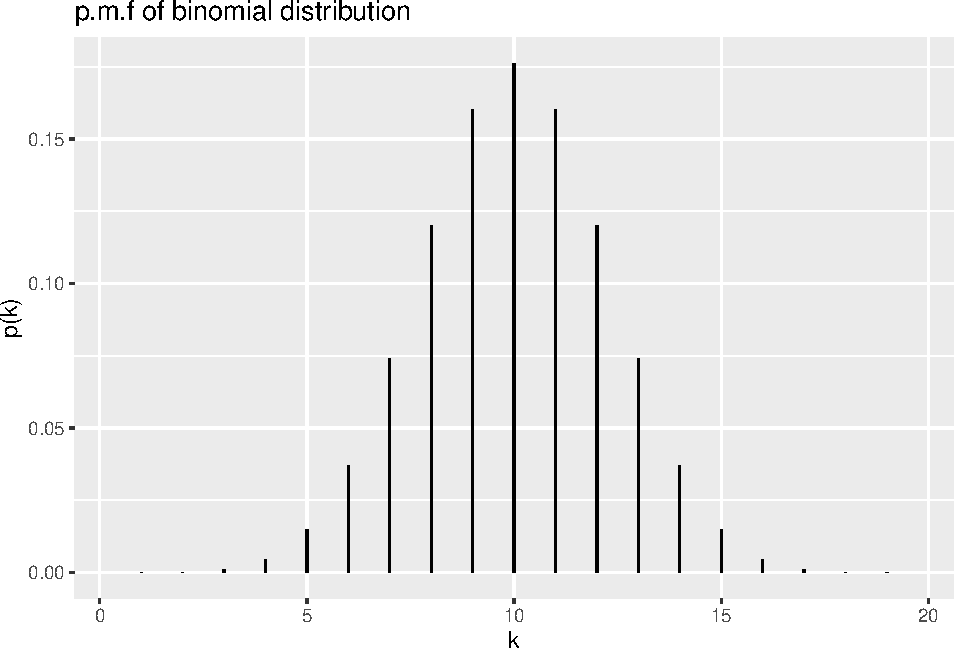
\includegraphics{SCMA470Bookdownproj_files/figure-latex/unnamed-chunk-1-1.pdf}

To plot continuous probability distribution in R, we use stat\_function to add the density function as its arguement. To specify a different mean or standard deviation, we use the \texttt{args} parameter to supply new values.

\begin{Shaded}
\begin{Highlighting}[]
\FunctionTok{library}\NormalTok{(ggplot2)}
\NormalTok{df }\OtherTok{\textless{}{-}} \FunctionTok{data.frame}\NormalTok{(}\AttributeTok{x=}\FunctionTok{seq}\NormalTok{(}\SpecialCharTok{{-}}\DecValTok{10}\NormalTok{,}\DecValTok{10}\NormalTok{,}\AttributeTok{by=}\FloatTok{0.1}\NormalTok{))}
\FunctionTok{ggplot}\NormalTok{(df) }\SpecialCharTok{+} 
    \FunctionTok{stat\_function}\NormalTok{(}\FunctionTok{aes}\NormalTok{(x),}\AttributeTok{fun=}\NormalTok{dnorm, }\AttributeTok{args =} \FunctionTok{list}\NormalTok{(}\AttributeTok{mean =} \DecValTok{0}\NormalTok{, }\AttributeTok{sd =} \DecValTok{1}\NormalTok{))  }\SpecialCharTok{+} 
    \FunctionTok{labs}\NormalTok{(}\AttributeTok{x =} \StringTok{"x"}\NormalTok{, }\AttributeTok{y =} \StringTok{"f(x)"}\NormalTok{, }
       \AttributeTok{title =} \StringTok{"Normal Distribution With Mean = 0 \& SD = 1"}\NormalTok{) }
\end{Highlighting}
\end{Shaded}

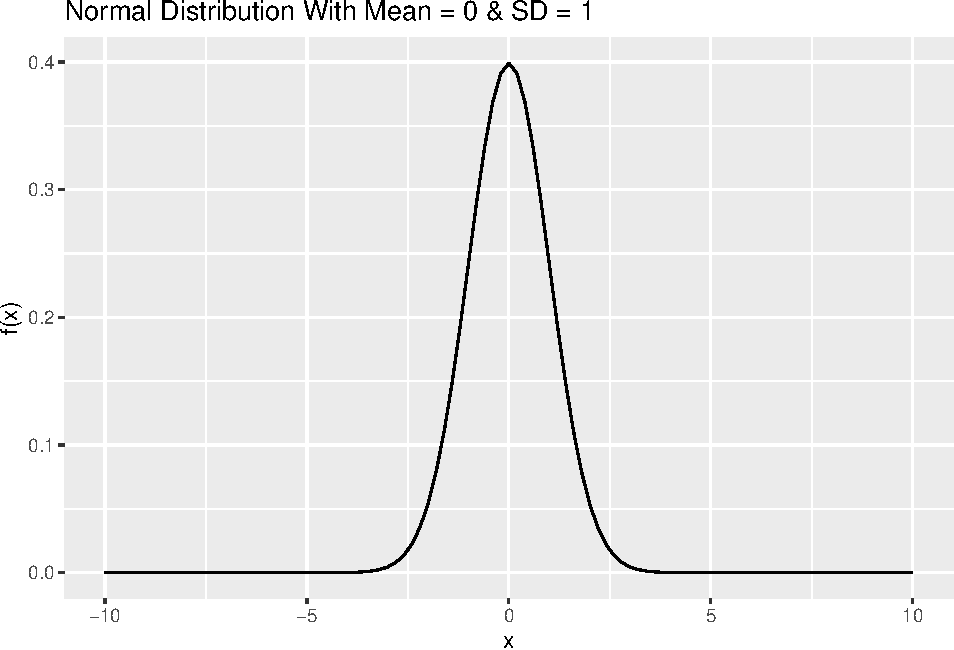
\includegraphics{SCMA470Bookdownproj_files/figure-latex/unnamed-chunk-2-1.pdf}

\hypertarget{expectation}{%
\section{Expectation}\label{expectation}}

\begin{definition}
\protect\hypertarget{def:unlabeled-div-5}{}\label{def:unlabeled-div-5}

\emph{The \textbf{expected value} of a discrete random variable
\(X\) with the set of possible values \(A\) and probability mass function
\(f(x)\) is defined by \[\mathrm{E}(X) = \sum_{x \in A} x f(x)\]}

\end{definition}

The \textbf{expected value} of a random variable \(X\) is also called the mean,
or the mathematical expectation, or simply the expectation of \(X\). It is
also occasionally denoted by \(\mathrm{E}[X]\), \(\mu_X\), or \(\mu\).

Note that if each value \(x\) of \(X\) is weighted by \(f(x) = P(X = x)\),
then \(\displaystyle \sum_{x \in A} x f(x)\) is nothing but the weighted
average of \(X\).

\begin{theorem}
\protect\hypertarget{thm:unlabeled-div-6}{}\label{thm:unlabeled-div-6}

\emph{Let \(X\) be a discrete random variable with set of
possible values \(A\) and probability mass function \(f(x)\), and let \(g\) be
a real-valued function. Then \(g(X)\) is a random variable with
\[\mathrm{E}[g(X)] = \sum_{x \in A} g(x) f(x)\] }

\end{theorem}

\begin{definition}
\protect\hypertarget{def:unlabeled-div-7}{}\label{def:unlabeled-div-7}

\emph{If \(X\) is a continuous random variable with
probability density function \(f\) , the \textbf{expected value} of \(X\) is
defined by \[\mathrm{E}(X) = \int_{-\infty}^\infty x f(x)\, dx\] }

\end{definition}

\begin{theorem}
\protect\hypertarget{thm:unlabeled-div-8}{}\label{thm:unlabeled-div-8}

\begin{itemize}
\tightlist
\item
  Let \(X\) be a continuous random variable with
  probability density function \(f (x)\); then for any function
  \(h: \mathbb{R} \rightarrow \mathbb{R}\),
  \[\mathrm{E}[h(X)] = \int_{-\infty}^\infty h(x)\, f(x)\, dx\] *
\end{itemize}

\end{theorem}

\begin{theorem}
\protect\hypertarget{thm:unlabeled-div-9}{}\label{thm:unlabeled-div-9}

\emph{Let \(X\) be a random variable. Let
\(h_1, h_2, . . . , h_n\) be real-valued functions, and
\(a_1, a_2, \ldots, a_n\) be real numbers. Then
\[\mathrm{E}[a_1 h_1(X) + a_2 h_2(X) + \cdots + a_n h_n(X)] = a_1 \mathrm{E}[h_1(X)] + a_2 \mathrm{E}[h_2(X)] + \ldots +
    a_n \mathrm{E}[h_n(X)]\]}

\end{theorem}

Moreover, if \(a\) and \(b\) are constants, then
\[\mathrm{E}(aX +b) = a\mathrm{E}(x) + b\]

\hypertarget{variances-of-random-variables}{%
\section{Variances of Random Variables}\label{variances-of-random-variables}}

\begin{definition}
\protect\hypertarget{def:unlabeled-div-10}{}\label{def:unlabeled-div-10}

\emph{Let \(X\) be a discrete random variable with a set of
possible values \(A\), probability mass function \(f(x)\), and
\(\mathrm{E}(X) = \mu\). then \(\mathrm{Var}(X)\) and \(\sigma_X\), called the
\textbf{variance} and \textbf{standard deviation} of \(X\), respectively, are
defined by
\[\mathrm{Var}(X) = \mathrm{E}[(X- \mu)^2] = \sum_{x \in A} (x - \mu)^2 f(x),\]
\[\sigma_X = \sqrt{\mathrm{E}[(X- \mu)^2]}\]}

\end{definition}

\begin{definition}
\protect\hypertarget{def:unlabeled-div-11}{}\label{def:unlabeled-div-11}

\emph{If \(X\) is a continuous random variable with
\(\mathrm{E}(X) = \mu\), then \(\mathrm{Var}(X)\) and \(\sigma_X\), called the
\textbf{variance} and \textbf{standard deviation} of \(X\), respectively, are
defined by
\[\mathrm{Var}(X) = \mathrm{E}[(X- \mu)^2] =  \int_{-\infty}^\infty (x - \mu)^2\, f(x)\, dx ,\]
\[\sigma_X = \sqrt{\mathrm{E}[(X- \mu)^2]}\]}

\end{definition}

We have the following important relations
\[\mathrm{Var}(x) = \mathrm{E}(X^2) - (\mathrm{E}(x))^2 ,\]
\[\mathrm{Var}(aX + b) = a^2\ Var(X), \quad   \sigma_{aX + b}= |a|\sigma_X\]
where \(a\) and \(b\) are constants.

\hypertarget{moments-and-moment-generating-function}{%
\section{Moments and Moment Generating Function}\label{moments-and-moment-generating-function}}

\begin{definition}
\protect\hypertarget{def:unlabeled-div-12}{}\label{def:unlabeled-div-12}

\emph{For \(r > 0\), the \(r\)th moment of \(X\) (the \(r\)th
moment about the origin) is \(\mathrm{E}[X^r]\), when it is defined. The
\(r\)th central moment of a random variable \(X\) (the \(r\)th moment about
the mean) is \(\mathrm{E}[(X - \mathrm{E}[X])^r].\) }

\end{definition}

\begin{definition}
\protect\hypertarget{def:unlabeled-div-13}{}\label{def:unlabeled-div-13}

\emph{The skewness of \(X\) is defined to be the third
central moment, \[\mathrm{E}[(X - \mathrm{E}[X])^3],\] and the
coefficient of skewness to be given by
\[\frac{\mathrm{E}[(X - \mathrm{E}[X])^3]}{(\mathrm{Var}[X])^{3/2}}.\] }

\end{definition}

\begin{definition}
\protect\hypertarget{def:unlabeled-div-14}{}\label{def:unlabeled-div-14}

\emph{The coefficient of kurtosis of \(X\) is defined by
\[\frac{\mathrm{E}[(X - \mathrm{E}[X])^4]}{(\mathrm{Var}[X])^{4/2}}.\] }

\end{definition}

\textbf{Note} In the formula, subtract from the mean and normalise or divide by the standard deviation center and scale to the standard values. Odd-order moments are increased if there is a long tail to the right and decreased if there is a long tail to the left, while even-order moments are increased if either tail is long. A negative value of the coefficient of skewness that the distribution is skewed to the left, or negatively skewed, meaning that the deviations above the mean tend to be smaller than the deviations below the mean, and vice versa. If the coefficent of skewness is close to zero, this could mean symmetry,

\textbf{Note} The fourth moment measures the fatness in the tails, which is always positive. The kurtosis of the standard normal distribution is 3. Using the standard normal distribution as a benchmark, the excess kurtosis of a random variable is defined as the kurtosis minus 3. A higher kurtosis corresponds to a larger extremity of deviations (or outliers), which is called excess kurtosis.

The following diagram compares the shape between the normal distribution and Student's t-distribution. Note that to use the legend with the \texttt{stat\_function} in ggplot2, we use \texttt{scale\_colour\_manual} along with \texttt{colour\ =} inside the \texttt{aes()} as shown below and give names for specific density plots.

\begin{Shaded}
\begin{Highlighting}[]
\FunctionTok{library}\NormalTok{(ggplot2)}
\NormalTok{df }\OtherTok{\textless{}{-}} \FunctionTok{data.frame}\NormalTok{(}\AttributeTok{x=}\FunctionTok{seq}\NormalTok{(}\SpecialCharTok{{-}}\DecValTok{10}\NormalTok{,}\DecValTok{10}\NormalTok{,}\AttributeTok{by=}\FloatTok{0.1}\NormalTok{))}
\FunctionTok{ggplot}\NormalTok{(df) }\SpecialCharTok{+} 
    \FunctionTok{stat\_function}\NormalTok{(}\FunctionTok{aes}\NormalTok{(x, }\AttributeTok{colour =} \StringTok{"dnorm"}\NormalTok{),}\AttributeTok{fun =}\NormalTok{ dnorm, }\AttributeTok{args =} \FunctionTok{list}\NormalTok{(}\AttributeTok{mean =} \DecValTok{0}\NormalTok{, }\AttributeTok{sd =} \DecValTok{1}\NormalTok{))  }\SpecialCharTok{+} 
    \FunctionTok{stat\_function}\NormalTok{(}\FunctionTok{aes}\NormalTok{(x, }\AttributeTok{colour =}\StringTok{"dt"}\NormalTok{),}\AttributeTok{fun =}\NormalTok{ dt, }\AttributeTok{args =} \FunctionTok{list}\NormalTok{(}\AttributeTok{df =} \DecValTok{4}\NormalTok{)) }\SpecialCharTok{+}
     \FunctionTok{scale\_colour\_manual}\NormalTok{(}\StringTok{"Legend title"}\NormalTok{, }\AttributeTok{values =} \FunctionTok{c}\NormalTok{(}\StringTok{"black"}\NormalTok{, }\StringTok{"blue"}\NormalTok{)) }\SpecialCharTok{+} 
    \FunctionTok{labs}\NormalTok{(}\AttributeTok{x =} \StringTok{"x"}\NormalTok{, }\AttributeTok{y =} \StringTok{"f(x)"}\NormalTok{, }
       \AttributeTok{title =} \StringTok{"Normal Distribution With Mean = 0 \& SD = 1"}\NormalTok{) }\SpecialCharTok{+} 
  \FunctionTok{theme}\NormalTok{(}\AttributeTok{plot.title =} \FunctionTok{element\_text}\NormalTok{(}\AttributeTok{hjust =} \FloatTok{0.5}\NormalTok{))}
\end{Highlighting}
\end{Shaded}

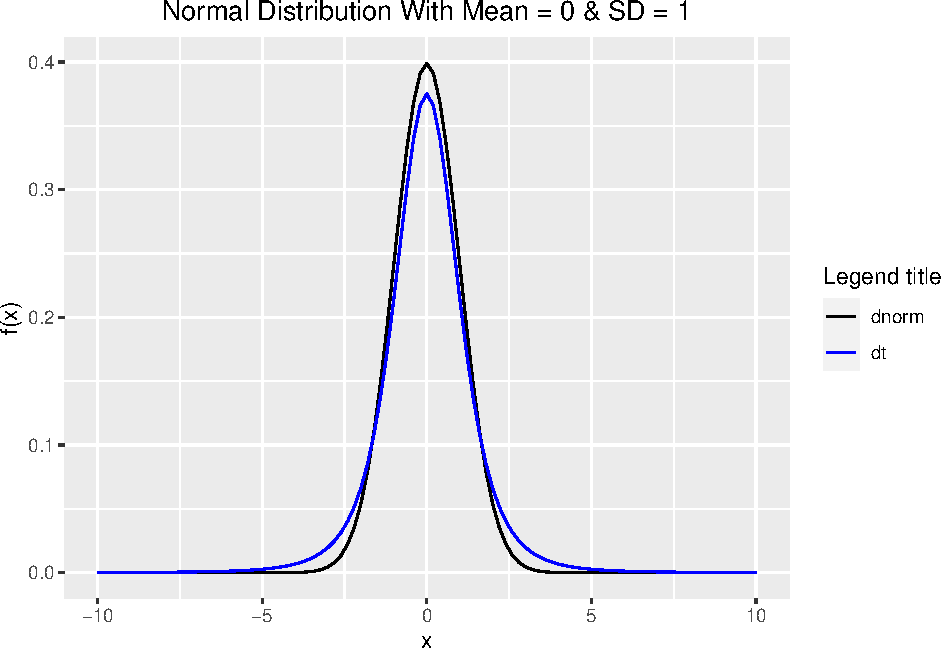
\includegraphics{SCMA470Bookdownproj_files/figure-latex/unnamed-chunk-3-1.pdf}

Next we will simulate 10000 samples from a normal distribution with mean 0, and standard deviation 1, then compute and interpret for the skewness and kurtosis, and plot the histogram. Here we also use
the function \texttt{set.seed()} to set the seed of R's random number generator, this is useful for creating simulations or random objects that can be reproduced.

\begin{Shaded}
\begin{Highlighting}[]
\FunctionTok{set.seed}\NormalTok{(}\DecValTok{15}\NormalTok{) }\CommentTok{\# Set the seed of R\textquotesingle{}s random number generator}

\CommentTok{\#Simulation}
\NormalTok{n.sample }\OtherTok{\textless{}{-}} \FunctionTok{rnorm}\NormalTok{(}\AttributeTok{n =} \DecValTok{10000}\NormalTok{, }\AttributeTok{mean =} \DecValTok{0}\NormalTok{, }\AttributeTok{sd =} \DecValTok{1}\NormalTok{)}

\CommentTok{\#Skewness and Kurtosis}
\FunctionTok{library}\NormalTok{(moments)}
\FunctionTok{skewness}\NormalTok{(n.sample)}
\end{Highlighting}
\end{Shaded}

\begin{verbatim}
## [1] -0.03585812
\end{verbatim}

\begin{Shaded}
\begin{Highlighting}[]
\FunctionTok{kurtosis}\NormalTok{(n.sample)}
\end{Highlighting}
\end{Shaded}

\begin{verbatim}
## [1] 2.963189
\end{verbatim}

\begin{Shaded}
\begin{Highlighting}[]
\FunctionTok{ggplot}\NormalTok{(}\FunctionTok{data.frame}\NormalTok{(}\AttributeTok{x =}\NormalTok{ n.sample),}\FunctionTok{aes}\NormalTok{(x)) }\SpecialCharTok{+} 
  \FunctionTok{geom\_histogram}\NormalTok{(}\AttributeTok{binwidth =} \FloatTok{0.5}\NormalTok{)}
\end{Highlighting}
\end{Shaded}

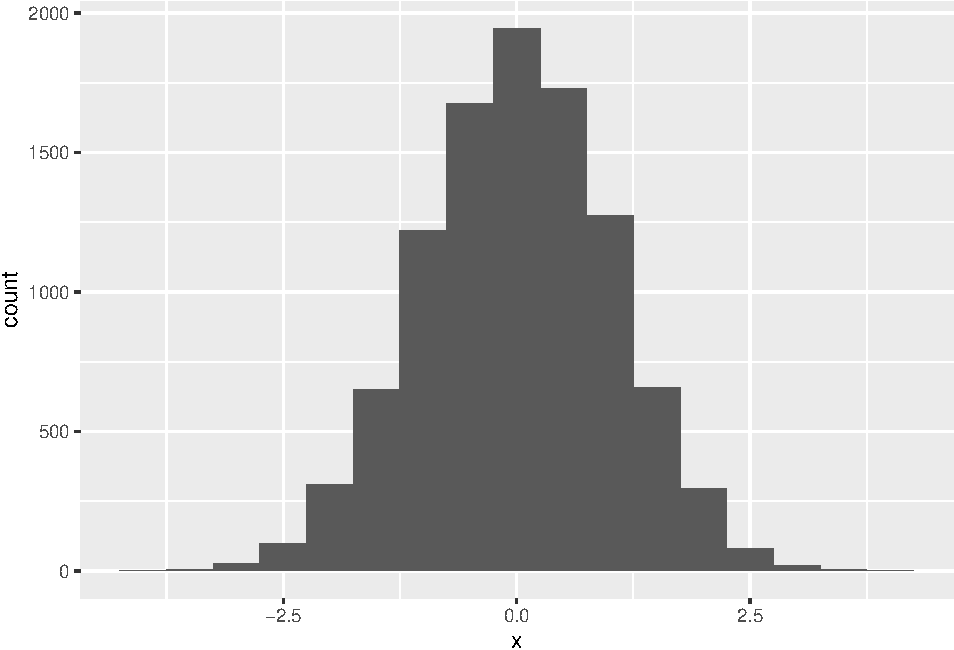
\includegraphics{SCMA470Bookdownproj_files/figure-latex/unnamed-chunk-4-1.pdf}

\begin{Shaded}
\begin{Highlighting}[]
\FunctionTok{set.seed}\NormalTok{(}\DecValTok{15}\NormalTok{)}

\CommentTok{\#Simulation}
\NormalTok{t.sample }\OtherTok{\textless{}{-}} \FunctionTok{rt}\NormalTok{(}\AttributeTok{n =} \DecValTok{10000}\NormalTok{, }\AttributeTok{df =} \DecValTok{5}\NormalTok{)}

\CommentTok{\#Skewness and Kurtosis}
\FunctionTok{library}\NormalTok{(moments)}
\FunctionTok{skewness}\NormalTok{(t.sample)}
\end{Highlighting}
\end{Shaded}

\begin{verbatim}
## [1] 0.06196269
\end{verbatim}

\begin{Shaded}
\begin{Highlighting}[]
\FunctionTok{kurtosis}\NormalTok{(t.sample)}
\end{Highlighting}
\end{Shaded}

\begin{verbatim}
## [1] 7.646659
\end{verbatim}

\begin{Shaded}
\begin{Highlighting}[]
\FunctionTok{ggplot}\NormalTok{(}\FunctionTok{data.frame}\NormalTok{(}\AttributeTok{x =}\NormalTok{ t.sample),}\FunctionTok{aes}\NormalTok{(x)) }\SpecialCharTok{+} \FunctionTok{geom\_histogram}\NormalTok{(}\AttributeTok{binwidth =} \FloatTok{0.5}\NormalTok{)}
\end{Highlighting}
\end{Shaded}

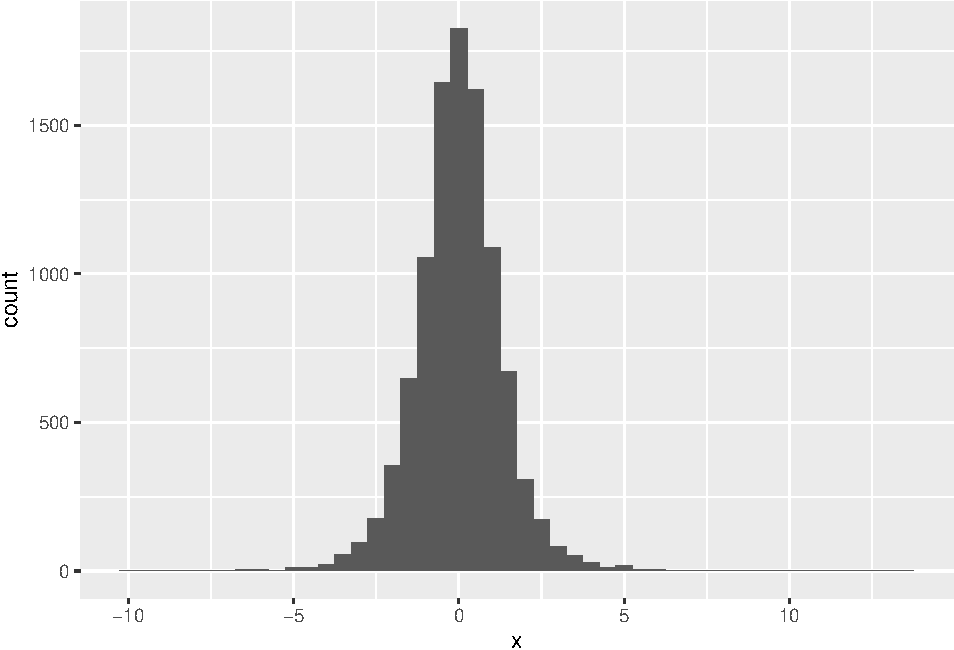
\includegraphics{SCMA470Bookdownproj_files/figure-latex/unnamed-chunk-5-1.pdf}

\textbf{Example} Let us count the number of samples greater than 5 from the samples of the normal and Student's t distributions. Comment on your results

eyJsYW5ndWFnZSI6InIiLCJzYW1wbGUiOiIjIFdyaXRlIHlvdXIgY29kZSBoZXJlXG5zZXQuc2VlZCgxNSlcbm4uc2FtcGxlIDwtIHJub3JtKG4gPSAxMDAwMCwgbWVhbiA9IDAsIHNkID0gMSlcbnQuc2FtcGxlIDwtIHJ0KG4gPSAxMDAwMCwgZGYgPSA1KSJ9

\begin{definition}
\protect\hypertarget{def:unlabeled-div-15}{}\label{def:unlabeled-div-15}

\emph{The moment generating function (mgf) of a random
variable \(X\) is defined to be \[M_X(t) = E[e^{tX}],\] if the expectation
exists.}

\end{definition}

\textbf{Note} The moment generating function of \(X\) may not defined (may not
be finite) for all \(t\) in \(\mathbb{R}\).

If \(M_X(t)\) is finite for \(|t| < h\) for some \(h > 0\), then, for any
\(k = 1, 2, \ldots,\) the function \(M_X(t)\) is k-times differentiable at
\(t = 0\), with \[M^{(k)}_X (0) = \mathrm{E}[X^k],\] with
\(\mathrm{E}[|X|^k]\) finite. We can obtain the moments by succesive
differentiation of \(M_X(t)\) and letting \(t = 0\).

\begin{example}
\protect\hypertarget{exm:unlabeled-div-16}{}\label{exm:unlabeled-div-16}

Derive the formula for the mgf of the standard normal distribution.
Hint: its mgf is \(e^{\frac{1}{2} t^2}\).

\end{example}

\hypertarget{probability-generating-function}{%
\section{Probability generating function}\label{probability-generating-function}}

\begin{definition}
\protect\hypertarget{def:unlabeled-div-17}{}\label{def:unlabeled-div-17}

\emph{For a counting variable \(N\) (a variable which
assumes some or all of the values \(0, 1, 2, \ldots,\) but no others), The
probability generating function of \(N\) is \[G_N(t) = E[t^N],\] for those
\(t\) in \(\mathbb{R}\) for which the series converges absolutely. }

\end{definition}

Let \(p_k = P(N = k)\). Then
\[G_N(t) = E[t^N] = \sum_{k=0}^\infty t^k p_k.\] It can be shown that if
\(E[N] < \infty\) then \[\mathrm{E}[N] = G'_N(1),\] and if
\(E[N^2] < \infty\) then
\[\mathrm{Var}[N] = G''_N(1) + G'_N(1) - (G'_N(1))^2.\] Moreover, when
both pgf and mgf of \(N\) are defined, we have
\[G_N(t) = M_N(\log(t)) \quad \text{ and } M_N(t) = G_N(e^t).\]

\hypertarget{multivariate-distributions}{%
\section{Multivariate Distributions}\label{multivariate-distributions}}

When \(X_1,X_2,\ldots ,X_n\) be random variables defined on the same
sample space, a multivariate probability density function or probability
mass function\\
\(f(x_1, x_2, \ldots x_n)\) can be defined. The following definitions can
be extended to more than two random variables and the case of discrete
random variables.

\begin{definition}
\protect\hypertarget{def:unlabeled-div-18}{}\label{def:unlabeled-div-18}

\emph{Two random variables \(X\) and \(Y\), defined on the
same sample space, have a continuous joint distribution if there exists
a nonnegative function of two variables, \(f(x, y)\) on
\(\mathbb{R} \times \mathbb{R}\) , such that for any region \(R\) in the
\(xy\)-plane that can be formed from rectangles by a countable number of
set operations, \[P((X, Y)  \in R) = \iint_R f(x,y) \, dx\, dy\] }

\end{definition}

The function \(f (x, y)\) is called the \textbf{joint probability density
function} of \(X\) and \(Y\).

Let \(X\) and \(Y\) have joint probability density function \(f (x, y)\). Let
\(f_Y\) be the probability density function of \(Y\) . To find \(f_Y\) in
terms of \(f\) , note that, on the one hand, for any subset \(B\) of \(R\),
\[P(Y \in B) = \int_B f_Y(y) \, dy,\] and on the other hand, we also
have
\[P(Y \in B) = P(X \in (-\infty, \infty), Y \in B) = \int_B \left(    \int_{-\infty}^\infty f(x,y)\, dx  \right) \, dy.\]

We have
\begin{equation} 
\label{eq:label} f_Y(y) =   \int_{-\infty}^\infty f(x,y)\, dx
\end{equation}
and
\begin{equation} 
\label{eq:label2}  f_X(x) =   \int_{-\infty}^\infty f(x,y)\, dy
\end{equation}

\begin{definition}
\protect\hypertarget{def:unlabeled-div-19}{}\label{def:unlabeled-div-19}

\emph{Let \(X\) and \(Y\) have joint probability density
function \(f (x, y)\); then the functions \(f_X\) and \(f_Y\) in} \eqref{eq:label} and \eqref{eq:label2}
\emph{are called,
respectively, the \textbf{marginal probability density functions} of \(X\) and
\(Y\) .}

\end{definition}

Let \(X\) and \(Y\) be two random variables (discrete, continuous, or
mixed). The \textbf{joint probability distribution function}, or \textbf{joint
cumulative probability distribution function}, or simply the joint
distribution of \(X\) and \(Y\), is defined by
\[F(t, u) = P(X \le t, Y \le u)\] for all \(t, u \in (-\infty, \infty)\).

The marginal probability distribution function of \(X\), \(F_X\), can be
found from \(F\) as follows:
\[F_X(t) = \lim_{n \rightarrow \infty} F(t,u)  = F(t, \infty)\] and
\[F_Y(u) = \lim_{n \rightarrow \infty}F(t,u)  = F( \infty, u)\]

The following relationship between \(f(x,y)\) and \(F(t,u)\) is as follows:
\[F(t,u) = \int_{-\infty}^{u}\int_{-\infty}^{t} f(x,y)\, dx\, dy.\]

We also have
\[\mathrm{E}(X) =   \int_{-\infty}^\infty x f_X(x)\, dx , \quad \mathrm{E}(Y) =   \int_{-\infty}^\infty y f_Y(y)\, dy\]

\begin{theorem}
\protect\hypertarget{thm:unlabeled-div-20}{}\label{thm:unlabeled-div-20}

\emph{Let \(f (x, y)\) be the joint probability density function
of random variables \(X\) and \(Y\). If \(h\) is a function of two variables
from \(\mathbb{R}^2\) to \(\mathbb{R}\), then \(h(X, Y )\) is a random
variable with the expected value given by
\[\mathrm{E}[h(X,Y)] = \int_{-\infty}^{\infty}\int_{-\infty}^{\infty} h(x,y) \, f(x,y)\, dx\, dy\]
provided that the integral is absolutely convergent.}

\end{theorem}

As a consequence of the above theorem, for random variables \(X\) and \(Y\),
\[\mathrm{E}(X + Y) = \mathrm{E}(X) + \mathrm{E}(Y)\]

\hypertarget{independent-random-variables}{%
\section{Independent random variables}\label{independent-random-variables}}

\begin{definition}
\protect\hypertarget{def:unlabeled-div-21}{}\label{def:unlabeled-div-21}

\emph{Two random variables \(X\) and \(Y\) are called
independent if, for arbitrary subsets \(A\) and \(B\) of real numbers, the
events \(\{X \in A\}\) and \(\{Y \in B\}\) are \textbf{independent}, that is, if
\[P(X \in A, Y \in B) = P(X \in A) P(Y \in B).\]}

\end{definition}

\begin{theorem}
\protect\hypertarget{thm:unlabeled-div-22}{}\label{thm:unlabeled-div-22}

\emph{Let \(X\) and \(Y\) be two random variables defined on the
same sample space. If \(F\) is the joint probability distribution function
of \(X\) and \(Y\), then \(X\) and \(Y\) are independent if and only if for all
real numbers \(t\) and \(u\), \[F(t,u)  = F_X(t) F_Y(u).\]}

\end{theorem}

\begin{theorem}
\protect\hypertarget{thm:unlabeled-div-23}{}\label{thm:unlabeled-div-23}

\emph{Let \(X\) and \(Y\) be jointly continuous random variables
with joint probability density function \(f (x, y)\). Then \(X\) and \(Y\) are
independent if and only if \[f (x, y) = f_X(x) f_Y (y).\]}

\end{theorem}

\begin{theorem}
\protect\hypertarget{thm:unlabeled-div-24}{}\label{thm:unlabeled-div-24}

\emph{Let \(X\) and \(Y\) be independent random variables and
\(g : \mathbb{R} \rightarrow\mathbb{R}\) and
\(h : \mathbb{R} \rightarrow\mathbb{R}\) be real-valued functions; then
\(g(X)\) and \(h(Y )\) are also independent random variables.}

\end{theorem}

As a consequence of the above theorem, we obtain

\begin{theorem}
\protect\hypertarget{thm:unlabeled-div-25}{}\label{thm:unlabeled-div-25}

\emph{Let \(X\) and \(Y\) be independent random variables. Then
for all real-value functions \(g : \mathbb{R} \rightarrow\mathbb{R}\) and
\(h : \mathbb{R} \rightarrow\mathbb{R}\),
\[\mathrm{E}[g(X)h(Y)] = \mathrm{E}[g(X)]\mathrm{E}[h(Y)]\] }

\end{theorem}

\hypertarget{conditional-distributions}{%
\section{Conditional Distributions}\label{conditional-distributions}}

Let \(X\) and \(Y\) be two continuous random variables with the joint
probability density function \(f (x, y)\). Note that the case of discrete
random variables can be considered in the same way. When no information
is given about the value of \(Y\), the marginal probability density
function of \(X\), \(f_X(x)\) is used to calculate the probabilities of
events concerning \(X\). However, when the value of \(Y\) is known, to find
such probabilities, \(f_{X|Y} (x|y)\), the conditional probability density
function of \(X\) given that \(Y = y\) is used and is defined as follows:
\[f_{X|Y} (x|y)  = \frac{f(x,y)}{f_Y(y)}\] provided that \(f_Y (y) > 0\).
Note also that the conditional probability density function of \(X\) given
that \(Y = y\) is itseof a probability density function, i.e.
\[\int_{-\infty}^\infty f_{X|Y}(x|y)\, dx  =  1.\]

Note that the conditional probability distribution function of \(X\) given
that \(Y = y\), the conditional expectation of \(X\) given that \(Y = y\) can
be as follows:
\[F_{Y|X}(x|y) = P(X \le x | Y = y) = \int_ {-\infty}^x f_{X|Y}(t|y) \, dt\]
and
\[\mathrm{E}(X|Y = y) =  \int_{-\infty}^{\infty} x  f_{X|Y}(x|y) \, dx,\]
where \(f_Y(y) > 0\).

Note that if \(X\) and \(Y\) are independent, then \(f_{X|Y}\) coincides with
\(f_X\) because
\[f_{X|Y}(x|y) = \frac{f(x,y)}{f_Y(y)} =\frac{f_X(x)f_Y(y)}{f_Y(y)} = f_X(x).\]

\hypertarget{covariance}{%
\section{Covariance}\label{covariance}}

The notion of the variance of a random variable \(X\),
\(\mathrm{Var}(X) = \mathrm{E}[ ( X - \mathrm{E}(X))^2]\) measures the
average magnitude of the fluctuations of the random variable \(X\) from
its expectation, \(\mathrm{E}(X)\). This quantity measures the dispersion,
or spread, of the distribution of \(X\) about its expectation. Now suppose
that \(X\) and \(Y\) are two jointly distributed random variables.
Covariance is a measure of how much two random variables vary together.

Let us calculuate \(\mathrm{Var}(aX + bY)\) the joint spread, or
dispersion, of \(X\) and \(Y\) along the \((ax + by)\)-direction for arbitrary
real numbers \(a\) and \(b\):
\[\mathrm{Var}(aX + bY) = a^2 \mathrm{Var}(X) + b^2 \mathrm{Var}(Y) + 2 a b \mathrm{E}[(X - \mathrm{E}(X))(Y - \mathrm{E}(Y))].\]
However, \(\mathrm{Var}(X)\) and \(\mathrm{Var}(Y )\) determine the
dispersions of \(X\) and \(Y\) independently; therefore,
\(\mathrm{E}[(X - \mathrm{E}(X))(Y - \mathrm{E}(Y))]\) is the quantity
that gives information about the joint spread, or dispersion, \(X\) and
\(Y\) .

\begin{definition}
\protect\hypertarget{def:unlabeled-div-26}{}\label{def:unlabeled-div-26}

\emph{Let \(X\) and \(Y\) be jointly distributed random
variables; then the \textbf{covariance} of \(X\) and \(Y\) is defined by
\[\mathrm{Cov}(X,Y) =  \mathrm{E}[(X - \mathrm{E}(X))(Y - \mathrm{E}(Y))].\]}

\end{definition}

Note that for random variables \(X, Y\) and \(Z\), and \(ab > 0\), then the
joint dispersion of \(X\) and \(Y\) along the \((ax + by)\)-direction is
greater than the joint dispersion of \(X\) and \(Z\) along the
\((ax + bz)\)-direction if and only if
\(\mathrm{Cov}(X, Y) > \mathrm{Cov}(X,Z).\)

Note that \[\mathrm{Cov}(X, X) = \mathrm{Var}(X).\] Moreover,
\[\mathrm{Cov}(X,Y) = \mathrm{E}(XY) - \mathrm{E}(X)\mathrm{E}(Y).\]

Properties of covariance are as follows: for arbitrary real numbers
\(a, b, c, d\) and random variables \(X\) and \(Y\),
\[\mathrm{Var}(aX + bY) = a^2 \mathrm{Var}(X) + b^2 \mathrm{Var}(Y) + 2 a b \mathrm{Cov}(X,Y).\]
\[\mathrm{Cov}(aX + b, cY + d) = acCov(X, Y)\] For random variables
\(X_1, X_2, . . . , X_n\) and \(Y_1, Y_2, . . . , Y_m\),
\[\mathrm{Cov}(\sum_{i=1}^n a_i X_i, \sum_{j=1}^m b_j Y_j) = \sum_{i=1}^n\sum_{j=1}^m a_i\,b_j\, \mathrm{Cov}(X_i,Y_j).\]

If \(\mathrm{Cov}(X, Y) > 0\), we say that \(X\) and \(Y\) are positively
correlated. If \(\mathrm{Cov}(X, Y) < 0\), we say that they are negatively
correlated. If \(\mathrm{Cov}(X, Y) = 0\), we say that \(X\) and \(Y\) are
uncorrelated.

If \(X\) and \(Y\) are independent, then \[\mathrm{Cov}(X,Y) = 0.\] However,
the converse of this is not true; that is, two dependent random
variables might be uncorrelated.

\hypertarget{correlation}{%
\section{Correlation}\label{correlation}}

A large covariance can mean a strong relationship between variables.
However, we cannot compare variances over data sets with different
scales. A weak covariance in one data set may be a strong one in a
different data set with different scales. The problem can be fixed by
dividing the covariance by the standard deviation to get the correlation
coefficient.

\begin{definition}
\protect\hypertarget{def:unlabeled-div-27}{}\label{def:unlabeled-div-27}

\emph{Let \(X\) and \(Y\) be two random variables with
\(0< \sigma^2_X, \sigma^2_Y < \infty\). The covariance between the
standardized \(X\) and the standardized \(Y\) is called the correlation
coefficient between \(X\) and \(Y\) and is denoted \(\rho = \rho(X,Y)\),
\[\rho(X,Y) = \frac{\mathrm{Cov}(X,Y)}{\sigma_X \sigma_Y}.\] }

\end{definition}

Note that

\begin{itemize}
\item
  \(\rho(X, Y ) > 0\) if and only if \(X\) and \(Y\) are positively
  correlated;
\item
  \(\rho(X, Y ) < 0\) if and only if \(X\) and \(Y\) are negatively
  correlated; and
\item
  \(\rho(X, Y ) = 0\) if and only if \(X\) and \(Y\) are uncorrelated.
\item
  \(\rho(X, Y )\) roughly measures the amount and the sign of linear
  relationship between \(X\) and \(Y\).
\end{itemize}

In the case of perfect linear relationship, we have
\(\rho(X, Y ) = \pm1\). A correlation of 0, i.e.~\(\rho(X, Y ) = 0\) does
not mean zero relationship between two variables; rather, it means zero
linear relationship.

Some importants properties of correlation are
\[-1 \le \rho(X, Y ) \le 1\]
\[\rho(a X + b, cY +d) = \text{sign}(ac) \rho(X, Y )\]

\hypertarget{model-fitting}{%
\section{Model Fitting}\label{model-fitting}}

The contents in this section are taken from Gray and Pitts.

To fit a parametric model, we have to calculate estimates of the unknown
parameters of the probability distribution. Various criteria are
available, including the method of moments, the method of maximum
likelihood, etc.

\hypertarget{the-method-of-moments}{%
\section{The method of moments}\label{the-method-of-moments}}

The method of moments leads to parameter estimates by simply matching
the moments of the model,
\(\mathrm{E}[X], \mathrm{E}[X^2], \mathrm{E}[X^3], \ldots ,\) in turn to
the required number of corresponding sample moments calculated from the
data \(x_1, x_2, \ldots , x_n\), where \(n\) is the number of observations
available. The sample moments are simply
\[\frac{1}{n}\sum_{i=1}^n x_i, \quad  \frac{1}{n}\sum_{i=1}^n  x^2_i, \quad \frac{1}{n}\sum_{i=1}^n x^3_i, \ldots.\]
It is often more convenient to match the mean and central moments, in
particular matching \(\mathrm{E}[X]\) to the sample mean \(\bar{x}\) and
\(\mathrm{Var}[X]\) to the sample variance
\[s^2 = \frac{1}{n-1}\sum_{i=1}^n (x_i - \bar{x})^2.\]

An estimate produced using the method of moments is called an MME, and
the MME of a parameter \(\theta\), say, is usually denoted
\(\tilde{\theta}\).

\hypertarget{the-method-of-maximum-likelihood}{%
\section{The method of maximum likelihood}\label{the-method-of-maximum-likelihood}}

The method of maximum likelihood is the most widely used method for
parameter estimation. The estimates it produces are those values of the
parameters which give the maximum value attainable by the likelihood
function, denoted \(L\), which is the joint probability mass or density
function for the data we have (under the chosen parametric
distribution), regarded as a function of the unknown parameters.

In practice, it is often easier to maximise the loglikelihood function,
which is the logarithm of the likelihood function, rather than the
likelihood itself. An estimate produced using the method of maximum
likelihood is called an MLE, and the MLE of a parameter \(\theta\), say,
is denoted \(\hat{\theta}\). MLEs have many desirable theoretical
properties, especially in the case of large samples.

In some simple cases we can derive MLE(s) analytically as explicit
functions of summaries of the data. Thus, suppose our data consist of a
random sample \(x_1, x_2, \ldots , x_n\), from a parametric distribution
whose parameter(s) we want to estimate. Some straightforward cases
include the following:

\begin{itemize}
\item
  the MLE of \(\lambda\) for a \(Poi(\lambda)\) distribution is the sample
  mean, that is \(\hat{\lambda} = \bar{x}\)
\item
  the MLE of \(\lambda\) for an \(Exp(\lambda)\) distribution is the
  reciprocal of the sample mean, that is \(\hat{\lambda} = 1/\bar{x}\)
\end{itemize}

\hypertarget{goodness-of-fit-tests}{%
\section{Goodness of fit tests}\label{goodness-of-fit-tests}}

We can assess how well the fitted distributions reflect the distribution
of the data in various ways. We should, of course, examine and compare
the tables of frequencies and, if appropriate, plot and compare
empirical distribution functions. More formally, we can perform certain
statistical tests. Here we will use the Pearson chi-square
goodness-of-fit criterion.

\hypertarget{the-pearson-chi-square-goodness-of-fit-criterion}{%
\section{the Pearson chi-square goodness-of-fit criterion}\label{the-pearson-chi-square-goodness-of-fit-criterion}}

We construct the test statistic \[\chi^2 = \frac{\sum(O - E)^2}{E},\]
where \(O\) is the observed frequency in a cell in the frequency table and
\(E\) is the fitted or expected frequency (the frequency expected in that
cell under the fitted model), and where we sum over all usable cells.

\textbf{The null hypothesis} is that the sample comes from a specified
distribution.

The value of the test statistic is then evaluated in one of two ways.

\begin{enumerate}
\def\labelenumi{\arabic{enumi}.}
\item
  We convert it to a \(P\)-value, which is a measure of the strength of
  the evidence against the hypothesis that the data do follow the
  fitted distribution. \textbf{If the \(P\)-value is small enough, we conclude
  that the data do not follow the fitted distribution -- we say ``the
  fitted distribution does not provide a good fit to the data'' (and
  quote the \(P\)-value in support of this conclusion)}.
\item
  We compare it with values in published tables of the distribution
  function of the appropriate \(\chi^2\) distribution, and if the value
  of the statistic is high enough to be in a tail of specified size of
  this reference distribution, we conclude that the fitted
  distribution does not provide a good fit to the data.
\end{enumerate}

\hypertarget{kolmogorov-smirnov-k-s-test.}{%
\section{Kolmogorov-Smirnov (K-S) test.}\label{kolmogorov-smirnov-k-s-test.}}

The K-S test statistic is the maximum difference between the values of
the ecdf of the sample and the cdf of the fully specified fitted
distribution.

The course does not emphasis on the Goodness of Fit Test. Please refer
to the reference text for more details.

\hypertarget{loss-distributions}{%
\chapter{Loss distributions}\label{loss-distributions}}

\hypertarget{introduction}{%
\section{Introduction}\label{introduction}}

The aim of the course is to provide a fundamental basis which applies
mainly in general insurance. General insurance companies' products are
short-term policies that can be purchased for a short period of time.
Examples of insurance products are

\begin{itemize}
\item
  motor insurance;
\item
  home insurance;
\item
  health insurance; and
\item
  travel insurance.
\end{itemize}

In case of an occurrence of an insured event, two important components
of financial losses which are of importance for management of an
insurance company are

\begin{itemize}
\item
  the number of claims; and
\item
  the amounts of those claims.
\end{itemize}

Mathematical and statistical techniques used to model these sources of
uncertainty will be discussed. This will enable insurance companies to

\begin{itemize}
\item
  calculate premium rates to charge policy holders; and
\item
  decide how much reserve should be set aside for the future payment
  of incurred claims.
\end{itemize}

In the chapter, statistical distributions and their properties which are
suitable for modelling claim sizes are reviewed. These distribution are
also known as loss distributions. In practice, the shape of loss
distributions are positive skew with a long right tail. The main
features of loss distributions include:

\begin{itemize}
\item
  having a few small claims;
\item
  rising to a peak;
\item
  tailing off gradually with a few very large claims.
\end{itemize}

\hypertarget{exponential-distribution}{%
\section{Exponential Distribution}\label{exponential-distribution}}

A random variable \(X\) has an exponential distribution with a parameter
\(\lambda > 0\), denoted by \(X \sim \text{Exp}(\lambda)\) if its
probability density function is given by
\[f_X(x) = \lambda e^{-\lambda x}, \quad x > 0.\]

\begin{example}
\protect\hypertarget{exm:unlabeled-div-28}{}\label{exm:unlabeled-div-28}

\emph{Let \(X \sim \text{Exp}(\lambda)\) and \(0 < a < b\).}

\begin{enumerate}
\def\labelenumi{\arabic{enumi}.}
\item
  \emph{Find the distribution \(F_X(x)\).}
\item
  \emph{Express \(P(a < X < B)\) in terms of \(f_X(x)\) and \(F_X(x)\).}
\item
  \emph{Show that the moment generating function of \(X\) is
  \[M_X(t) = \left(1 -  \frac{t}{\lambda}\right)^{-1}, \quad t < \lambda.\]}
\item
  \emph{Derive the \(r\)-th moment about the origin \(\mathrm{E}[X^r].\)}
\item
  \emph{Derive the coefficient of skewness for \(X\).}
\item
  \emph{Simulate a random sample of size n = 200 from
  \(X \sim \text{Exp}(0.5)\) using the command
  \texttt{sample\ =\ rexp(n,\ rate\ =\ lambda)} where \(n\) and \(\lambda\) are the chosen
  parameter values.}
\item
  \emph{Plot a histogram of the random sample using the command
  \texttt{hist(sample)} (use help for available options for \texttt{hist} function
  in R).}
\end{enumerate}

\end{example}

\textbf{Solution:}
The code for questions 6 and 7 is given below. The histogram can be generated from the code below.

\begin{verbatim}
# set.seed is used so that random number generated from different simulations are the same. 
# The number 5353 can be set arbitrarily. 
set.seed(5353)

nsample <- 200
data_exp <- rexp(nsample, rate = 0.5)

dataset <- data_exp
hist(dataset, breaks=100,probability = TRUE, xlab = "claim sizes" 
     , ylab = "density", main = paste("Histogram of claim sizes" ))

hist(dataset, breaks=100, xlab = "claim sizes" 
     , ylab = "count", main = paste("Histogram of claim sizes" ))
\end{verbatim}

Copy and paste the code above and run it.

eyJsYW5ndWFnZSI6InIiLCJzYW1wbGUiOiJzZXQuc2VlZCg1MzUzKVxuXG5uc2FtcGxlIDwtIDIwMFxuZGF0YV9leHAgPC0gcmV4cChuc2FtcGxlLCByYXRlID0gMC41KVxuXG5kYXRhc2V0IDwtIGRhdGFfZXhwXG5oaXN0KGRhdGFzZXQsIGJyZWFrcz0xMDAscHJvYmFiaWxpdHkgPSBUUlVFLCB4bGFiID0gXCJjbGFpbSBzaXplc1wiIFxuICAgICAsIHlsYWIgPSBcImRlbnNpdHlcIiwgbWFpbiA9IHBhc3RlKFwiSGlzdG9ncmFtIG9mIGNsYWltIHNpemVzXCIgKSkifQ==

eyJsYW5ndWFnZSI6InIiLCJzYW1wbGUiOiJzZXQuc2VlZCg1MzUzKVxuXG5uc2FtcGxlIDwtIDIwMFxuZGF0YV9leHAgPC0gcmV4cChuc2FtcGxlLCByYXRlID0gMC41KVxuXG5kYXRhc2V0IDwtIGRhdGFfZXhwXG5cblxuaGlzdChkYXRhc2V0LCBicmVha3M9MTAwLCB4bGFiID0gXCJjbGFpbSBzaXplc1wiIFxuICAgICAsIHlsYWIgPSBcImNvdW50XCIsIG1haW4gPSBwYXN0ZShcIkhpc3RvZ3JhbSBvZiBjbGFpbSBzaXplc1wiICkpIn0=

\textbf{Notes}

\begin{enumerate}
\def\labelenumi{\arabic{enumi}.}
\item
  The exponential distribution can used to model the inter-arrival
  time of an event.
\item
  The exponential distribution has an important property called \textbf{lack
  of memory}: if \(X \sim \text{Exp}(\lambda)\), then the random
  variable \(X-w\) conditional on \(X > w\) has the same distribution as
  \(X\), i.e.
  \[X \sim \text{Exp}(\lambda)\Rightarrow  X - w | X > w \sim \text{Exp}(\lambda).\]
\end{enumerate}

We can use R to plot the probability density functions (pdf) of exponential distributions with various parameters \(\lambda\), which are shown in Figure \ref{fig:FigExp}. Here we use \texttt{scale\_colour\_manual} to override defaults with scales package (see cheat sheet for details).

\begin{Shaded}
\begin{Highlighting}[]
\FunctionTok{library}\NormalTok{(ggplot2)}
\FunctionTok{ggplot}\NormalTok{(}\FunctionTok{data.frame}\NormalTok{(}\AttributeTok{x=}\FunctionTok{c}\NormalTok{(}\DecValTok{0}\NormalTok{,}\DecValTok{10}\NormalTok{)), }\FunctionTok{aes}\NormalTok{(}\AttributeTok{x=}\NormalTok{x)) }\SpecialCharTok{+} 
  \FunctionTok{labs}\NormalTok{(}\AttributeTok{y=}\StringTok{"Probability density"}\NormalTok{, }\AttributeTok{x =} \StringTok{"x"}\NormalTok{) }\SpecialCharTok{+}
  \FunctionTok{ggtitle}\NormalTok{(}\StringTok{"Exponential distributions"}\NormalTok{) }\SpecialCharTok{+}
  \FunctionTok{theme}\NormalTok{(}\AttributeTok{plot.title =} \FunctionTok{element\_text}\NormalTok{(}\AttributeTok{hjust =} \FloatTok{0.5}\NormalTok{)) }\SpecialCharTok{+}
  \FunctionTok{stat\_function}\NormalTok{(}\AttributeTok{fun=}\NormalTok{dexp,}\AttributeTok{geom =}\StringTok{"line"}\NormalTok{, }\AttributeTok{args =}\NormalTok{ (}\AttributeTok{mean=}\FloatTok{0.5}\NormalTok{), }\FunctionTok{aes}\NormalTok{(}\AttributeTok{colour =} \StringTok{"0.5"}\NormalTok{)) }\SpecialCharTok{+}
  \FunctionTok{stat\_function}\NormalTok{(}\AttributeTok{fun=}\NormalTok{dexp,}\AttributeTok{geom =}\StringTok{"line"}\NormalTok{, }\AttributeTok{args =}\NormalTok{ (}\AttributeTok{mean=}\DecValTok{1}\NormalTok{), }\FunctionTok{aes}\NormalTok{(}\AttributeTok{colour =} \StringTok{"1"}\NormalTok{)) }\SpecialCharTok{+}
  \FunctionTok{stat\_function}\NormalTok{(}\AttributeTok{fun=}\NormalTok{dexp,}\AttributeTok{geom =}\StringTok{"line"}\NormalTok{, }\AttributeTok{args =}\NormalTok{ (}\AttributeTok{mean=}\FloatTok{1.5}\NormalTok{), }\FunctionTok{aes}\NormalTok{(}\AttributeTok{colour =} \StringTok{"1.5"}\NormalTok{)) }\SpecialCharTok{+}
  \FunctionTok{stat\_function}\NormalTok{(}\AttributeTok{fun=}\NormalTok{dexp,}\AttributeTok{geom =}\StringTok{"line"}\NormalTok{, }\AttributeTok{args =}\NormalTok{ (}\AttributeTok{mean=}\DecValTok{2}\NormalTok{), }\FunctionTok{aes}\NormalTok{(}\AttributeTok{colour =} \StringTok{"2"}\NormalTok{)) }\SpecialCharTok{+} 
  \FunctionTok{scale\_colour\_manual}\NormalTok{(}\FunctionTok{expression}\NormalTok{(}\FunctionTok{paste}\NormalTok{(lambda, }\StringTok{" = "}\NormalTok{)), }\AttributeTok{values =} \FunctionTok{c}\NormalTok{(}\StringTok{"red"}\NormalTok{, }\StringTok{"blue"}\NormalTok{, }\StringTok{"green"}\NormalTok{, }\StringTok{"orange"}\NormalTok{))}
\end{Highlighting}
\end{Shaded}

\begin{figure}
\centering
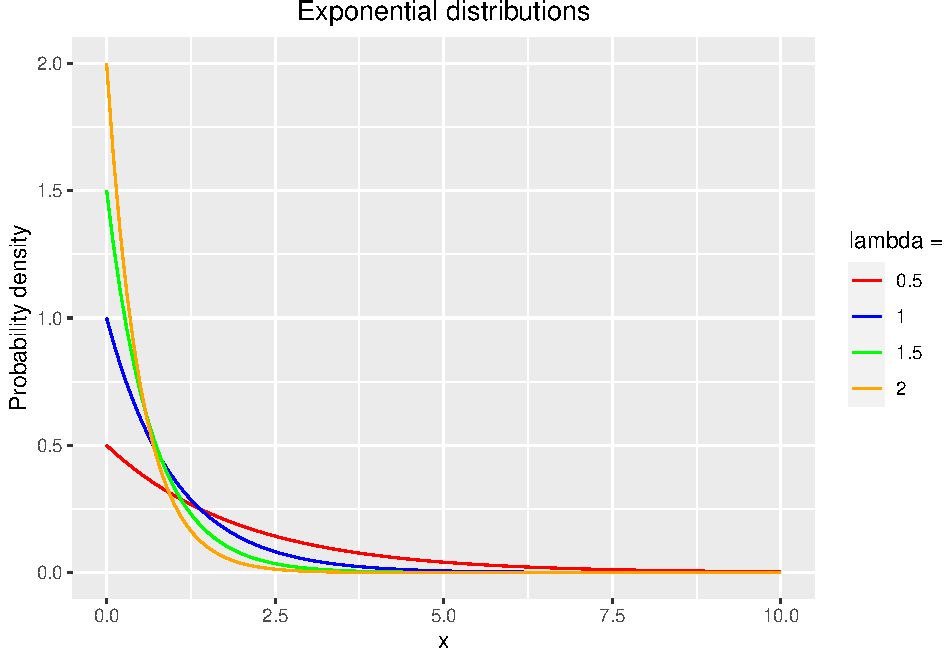
\includegraphics{SCMA470Bookdownproj_files/figure-latex/FigExp-1.pdf}
\caption{\label{fig:FigExp}The probability density functions (pdf) of exponential distributions with various parameters lambda.}
\end{figure}

\hypertarget{gamma-distribution}{%
\section{Gamma distribution}\label{gamma-distribution}}

A random variable \(X\) has a gamma distribution with parameters
\(\alpha > 0\) and \(\lambda > 0\), denoted by
\(X \sim \mathcal{G}(\alpha, \lambda)\) or
\(X \sim \text{gamma}(\alpha, \lambda)\) if its probability density
function is given by
\[f_X(x) = \frac{\lambda^\alpha}{\Gamma(\alpha)} x^{\alpha -1} e^{-\lambda x}, \quad x > 0.\]
The symbol \(\Gamma\) denotes the gamma function, which is defined as
\[\Gamma(\alpha) = \int_{0}^\infty x^{\alpha - 1} e^{-x} \mathop{}\!dx, \quad \text{for } \alpha > 0.\]
It follows that \(\Gamma(\alpha + 1) = \alpha \Gamma(\alpha)\) and that
for a positive integer \(n\), \(\Gamma(n) = (n-1)!\).

The properties of the gamma distribution are summarised.

\begin{itemize}
\item
  The mean and variance of \(X\) are
  \[\mathrm{E}[X] = \frac{\alpha}{\lambda} \text{ and } \mathrm{Var}[X] =\frac{\alpha}{\lambda^2}\]
\item
  The \(r\)-th moment about the origin is
  \[\mathrm{E}[X^r] = \frac{1}{\lambda^r} \frac{\Gamma(\alpha + r)}{\Gamma(\alpha )}, \quad r > 0.\]
\item
  The moment generating function (mgf) of \(X\) is
  \[M_X(t) = \left(1 -  \frac{t}{\lambda}\right)^{-\alpha}, \quad t < \lambda.\]
\item
  The coefficient of skewness is \[\frac{2}{\sqrt{\alpha}}.\]
\end{itemize}

\textbf{Notes}
1. The exponential function is a special case of the gamma
distribution, i.e.~\(\text{Exp}(\lambda)= \mathcal{G}(1,\lambda)\)

\begin{enumerate}
\def\labelenumi{\arabic{enumi}.}
\setcounter{enumi}{1}
\item
  If \(\alpha\) is a positive integer, the sum of \(\alpha\) independent,
  identically distributed as \(\text{Exp}(\lambda)\), is
  \(\mathcal{G}(\alpha, \lambda)\).
\item
  If \(X_1, X_2, \ldots, X_n\) are independent, identically distributed,
  each with a \(\mathcal{G}(\alpha, \lambda)\) distribution, then
  \[\sum_{i = 1}^n X_i \sim \mathcal{G}(n\alpha, \lambda).\]
\item
  The exponential and gamma distributions are not fat-tailed, and
  \textbf{may not provide a good fit} to claim amounts.
\end{enumerate}

\begin{example}
\protect\hypertarget{exm:unlabeled-div-29}{}\label{exm:unlabeled-div-29}

\emph{Using the moment generating function of a gamma
distribution, show that the sum of independent gamma random variables
with the same scale parameter \(\lambda\),
\(X \sim \mathcal{G}(\alpha_1, \lambda)\) and
\(Y \sim \mathcal{G}(\alpha_2, \lambda)\), is
\(S = X+ Y \sim \mathcal{G}(\alpha_1 + \alpha_2, \lambda).\)}

\end{example}

\textbf{Solution:}
Because \(X\) and \(Y\) are independent, \[\begin{aligned}
    M_S(t) &= M_{X+Y}(t) = M_X(t) \cdot M_Y(t)\\
        &= (1 - \frac{t}{\lambda})^{-\alpha_1} \cdot (1 - \frac{t}{\lambda})^{-\alpha_2}     \\
        &=  (1 - \frac{t}{\lambda})^{-(\alpha_1 + \alpha_2)}. \end{aligned}\]
Hence \(S = X + Y \sim \mathcal{G}(\alpha_1 + \alpha_2, \lambda).\)

The probability density functions (pdf) of gamma distributions with
various shape parameters \(\alpha\) and rate parameter \(\lambda\) = 1 are shown in Figure \ref{fig:FigGamma}.

\begin{Shaded}
\begin{Highlighting}[]
\FunctionTok{ggplot}\NormalTok{(}\FunctionTok{data.frame}\NormalTok{(}\AttributeTok{x=}\FunctionTok{c}\NormalTok{(}\DecValTok{0}\NormalTok{,}\DecValTok{20}\NormalTok{)), }\FunctionTok{aes}\NormalTok{(}\AttributeTok{x=}\NormalTok{x)) }\SpecialCharTok{+}
  \FunctionTok{labs}\NormalTok{(}\AttributeTok{y=}\StringTok{"Probability density"}\NormalTok{, }\AttributeTok{x =} \StringTok{"x"}\NormalTok{) }\SpecialCharTok{+} 
  \FunctionTok{ggtitle}\NormalTok{(}\StringTok{"Gamma distribution"}\NormalTok{)  }\SpecialCharTok{+}
  \FunctionTok{theme}\NormalTok{(}\AttributeTok{plot.title =} \FunctionTok{element\_text}\NormalTok{(}\AttributeTok{hjust =} \FloatTok{0.5}\NormalTok{)) }\SpecialCharTok{+}
  \FunctionTok{stat\_function}\NormalTok{(}\AttributeTok{fun=}\NormalTok{dgamma, }\AttributeTok{args=}\FunctionTok{list}\NormalTok{(}\AttributeTok{shape=}\DecValTok{2}\NormalTok{, }\AttributeTok{rate=}\DecValTok{1}\NormalTok{), }\FunctionTok{aes}\NormalTok{(}\AttributeTok{colour =} \StringTok{"2"}\NormalTok{)) }\SpecialCharTok{+}
  \FunctionTok{stat\_function}\NormalTok{(}\AttributeTok{fun=}\NormalTok{dgamma, }\AttributeTok{args=}\FunctionTok{list}\NormalTok{(}\AttributeTok{shape=}\DecValTok{6}\NormalTok{, }\AttributeTok{rate=}\DecValTok{1}\NormalTok{) , }\FunctionTok{aes}\NormalTok{(}\AttributeTok{colour =} \StringTok{"6"}\NormalTok{)) }\SpecialCharTok{+}
  \FunctionTok{scale\_colour\_manual}\NormalTok{(}\FunctionTok{expression}\NormalTok{(}\FunctionTok{paste}\NormalTok{(lambda, }\StringTok{" = 1 and "}\NormalTok{, alpha ,}\StringTok{" = "}\NormalTok{)), }\AttributeTok{values =} \FunctionTok{c}\NormalTok{(}\StringTok{"red"}\NormalTok{, }\StringTok{"blue"}\NormalTok{))}
\end{Highlighting}
\end{Shaded}

\begin{figure}
\centering
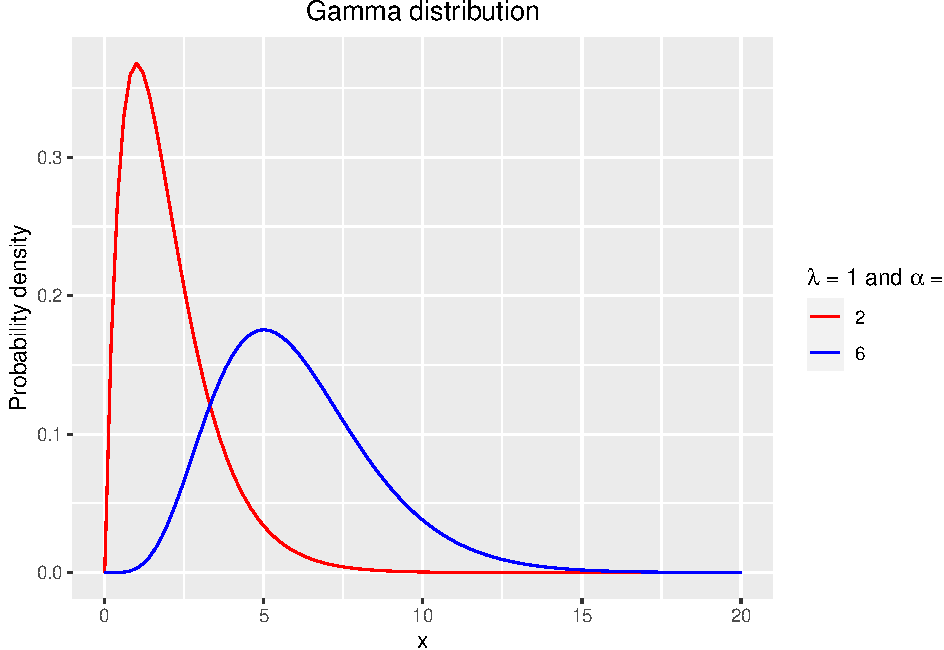
\includegraphics{SCMA470Bookdownproj_files/figure-latex/FigGamma-1.pdf}
\caption{\label{fig:FigGamma}The probability density functions (pdf) of gamma distributions with various shape alpha and rate parameter lambda = 1.}
\end{figure}

\hypertarget{lognormal-distribution}{%
\section{Lognormal distribution}\label{lognormal-distribution}}

A random variable \(X\) has a lognormal distribution with parameters \(\mu\)
and \(\sigma^2\), denoted by \(X \sim \mathcal{LN}(\mu, \sigma^2)\) if its
probability density function is given by
\[f_X(x) = \frac{1}{\sigma x \sqrt{2 \pi}} \exp\left(-\frac{1}{2} \left( \frac{\log(x) - \mu}{\sigma} \right)^2 \right) , \quad x > 0.\]

The following relation holds:
\[X \sim \mathcal{LN}(\mu, \sigma^2)\Leftrightarrow Y = \log X \sim \mathcal{N}(\mu, \sigma^2).\]

The properties of the lognormal distribution are summarised.

\begin{itemize}
\item
  The mean and variance of \(X\) are
  \[\mathrm{E}[X] = \exp\left(\mu + \frac{1}{2} \sigma^2 \right) \text{ and } \mathrm{Var}[X] =\exp\left(2\mu +  \sigma^2 \right) (\exp(\sigma^2) - 1).\]
\item
  The \(r\)-th moment about the origin is
  \[\mathrm{E}[X^r] =\exp\left(r\mu +  \frac{1}{2}r^2 \sigma^2 \right).\]
\item
  The moment generating function (mgf) of \(X\) is not finite for any
  positive value of \(t\).
\item
  The coefficient of skewness is
  \[(\exp(\sigma^2)  + 2) \left(\exp(\sigma^2)  -1 \right)^{1/2} .\]
\end{itemize}

The probability density functions (pdf) of gamma distributions with
various shape parameters \(\alpha\) and rate parameter \(\lambda = 1\) is shown in Figure \ref{fig:FigLognormal}.

\begin{Shaded}
\begin{Highlighting}[]
\FunctionTok{ggplot}\NormalTok{(}\FunctionTok{data.frame}\NormalTok{(}\AttributeTok{x=}\FunctionTok{c}\NormalTok{(}\DecValTok{0}\NormalTok{,}\DecValTok{10}\NormalTok{)), }\FunctionTok{aes}\NormalTok{(}\AttributeTok{x=}\NormalTok{x)) }\SpecialCharTok{+}
  \FunctionTok{labs}\NormalTok{(}\AttributeTok{y=}\StringTok{"Probability density"}\NormalTok{, }\AttributeTok{x =} \StringTok{"x"}\NormalTok{) }\SpecialCharTok{+} 
  \FunctionTok{ggtitle}\NormalTok{(}\StringTok{"lognormal distribution"}\NormalTok{)  }\SpecialCharTok{+}
  \FunctionTok{theme}\NormalTok{(}\AttributeTok{plot.title =} \FunctionTok{element\_text}\NormalTok{(}\AttributeTok{hjust =} \FloatTok{0.5}\NormalTok{)) }\SpecialCharTok{+}
  \FunctionTok{stat\_function}\NormalTok{(}\AttributeTok{fun=}\NormalTok{dlnorm, }\AttributeTok{args =} \FunctionTok{list}\NormalTok{(}\AttributeTok{meanlog =} \DecValTok{0}\NormalTok{, }\AttributeTok{sdlog =} \FloatTok{0.25}\NormalTok{), }\FunctionTok{aes}\NormalTok{(}\AttributeTok{colour =} \StringTok{"0.25"}\NormalTok{)) }\SpecialCharTok{+}
  \FunctionTok{stat\_function}\NormalTok{(}\AttributeTok{fun=}\NormalTok{dlnorm, }\AttributeTok{args =} \FunctionTok{list}\NormalTok{(}\AttributeTok{meanlog =} \DecValTok{0}\NormalTok{, }\AttributeTok{sdlog =} \DecValTok{1}\NormalTok{), }\FunctionTok{aes}\NormalTok{(}\AttributeTok{colour =} \StringTok{"1"}\NormalTok{)) }\SpecialCharTok{+}
  \FunctionTok{scale\_colour\_manual}\NormalTok{(}\FunctionTok{expression}\NormalTok{(}\FunctionTok{paste}\NormalTok{(mu, }\StringTok{" = 0 and "}\NormalTok{, sigma, }\StringTok{"= "}\NormalTok{)), }\AttributeTok{values =} \FunctionTok{c}\NormalTok{(}\StringTok{"red"}\NormalTok{, }\StringTok{"blue"}\NormalTok{))}
\end{Highlighting}
\end{Shaded}

\begin{figure}
\centering
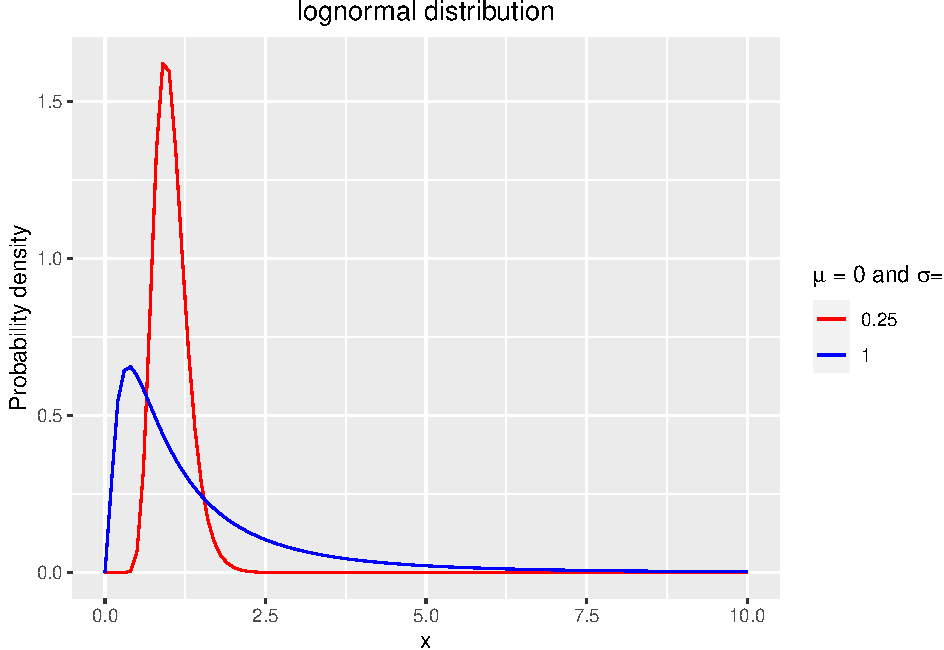
\includegraphics{SCMA470Bookdownproj_files/figure-latex/FigLognormal-1.pdf}
\caption{\label{fig:FigLognormal}The probability density functions (pdf) of lognormal distributions with mu = 0 and sigma = 0.25 or 1.}
\end{figure}

\hypertarget{pareto-distribution}{%
\section{Pareto distribution}\label{pareto-distribution}}

A random variable \(X\) has a Pareto distribution with parameters
\(\alpha > 0\) and \(\lambda > 0\), denoted by
\(X \sim \text{Pa}(\alpha, \lambda)\) if its probability density function
is given by
\[f_X(x) = \frac{\alpha \lambda^\alpha}{(\lambda + x)^{\alpha + 1}}, \quad x > 0.\]
The distribution function is given by
\[F_X(x) = 1 - \left(  \frac{\lambda}{\lambda + \alpha} \right)^\alpha, \quad x > 0.\]

The properties of the Pareto distribution are summarized.

\begin{itemize}
\item
  The mean and variance of \(X\) are
  \[\mathrm{E}[X] = \frac{\lambda}{\alpha - 1}, \alpha > 1 \text{ and } \mathrm{Var}[X] = \frac{\alpha \lambda^2}{(\alpha - 1)^2(\alpha - 2)}, \alpha > 2.\]
\item
  The \(r\)-th moment about the origin is
  \[\mathrm{E}[X^r] =\frac{\Gamma(\alpha-r) \Gamma(1+ r)}{\Gamma(\alpha)} \lambda^r, \quad 0 < r < \alpha.\]
\item
  The moment generating function (mgf) of \(X\) is not finite for any
  positive value of \(t\).
\item
  The coefficient of skewness is
  \[\frac{2(\alpha + 1)}{\alpha - 3} \sqrt{\frac{\alpha-2}{\alpha}} , \quad \alpha > 3.\]
\end{itemize}

\textbf{Note}
1. The following conditional tail property for a Pareto distribution is
useful for reinsurance calculation. Let
\(X \sim \text{Pa}(\alpha, \lambda)\). Then the random variable
\(X - w\) conditional on \(X > w\) has a Pareto distribution with
parameters \(\alpha\) and \(\lambda + w\), i.e.
\[X \sim \text{Pa}(\alpha, \lambda)\Rightarrow  X - w | X > w \sim \text{Pa}(\alpha,\lambda + w).\]

\begin{enumerate}
\def\labelenumi{\arabic{enumi}.}
\setcounter{enumi}{1}
\item
  The lognormal and Pareto distributions, in practice, provide a
  better fit to claim amounts than exponential and gamma
  distributions.
\item
  Other loss distribution are useful in practice including \textbf{Burr,
  Weibull and loggamma distributions}.
\end{enumerate}

\begin{Shaded}
\begin{Highlighting}[]
\FunctionTok{library}\NormalTok{(actuar)}
\FunctionTok{ggplot}\NormalTok{(}\FunctionTok{data.frame}\NormalTok{(}\AttributeTok{x=}\FunctionTok{c}\NormalTok{(}\DecValTok{0}\NormalTok{,}\DecValTok{60}\NormalTok{)), }\FunctionTok{aes}\NormalTok{(}\AttributeTok{x=}\NormalTok{x)) }\SpecialCharTok{+}
  \FunctionTok{labs}\NormalTok{(}\AttributeTok{y=}\StringTok{"Probability density"}\NormalTok{, }\AttributeTok{x =} \StringTok{"x"}\NormalTok{) }\SpecialCharTok{+} 
  \FunctionTok{ggtitle}\NormalTok{(}\StringTok{"Pareto distribution"}\NormalTok{)  }\SpecialCharTok{+}
  \FunctionTok{theme}\NormalTok{(}\AttributeTok{plot.title =} \FunctionTok{element\_text}\NormalTok{(}\AttributeTok{hjust =} \FloatTok{0.5}\NormalTok{)) }\SpecialCharTok{+}
  \FunctionTok{stat\_function}\NormalTok{(}\AttributeTok{fun=}\NormalTok{dpareto, }\AttributeTok{args=}\FunctionTok{list}\NormalTok{(}\AttributeTok{shape=}\DecValTok{3}\NormalTok{, }\AttributeTok{scale=}\DecValTok{20}\NormalTok{), }\FunctionTok{aes}\NormalTok{(}\AttributeTok{colour =} \StringTok{"alpha = 3, lambda = 20"}\NormalTok{)) }\SpecialCharTok{+}
  \FunctionTok{stat\_function}\NormalTok{(}\AttributeTok{fun=}\NormalTok{dpareto, }\AttributeTok{args=}\FunctionTok{list}\NormalTok{(}\AttributeTok{shape=}\DecValTok{6}\NormalTok{, }\AttributeTok{scale=}\DecValTok{50}\NormalTok{), }\FunctionTok{aes}\NormalTok{(}\AttributeTok{colour =} \StringTok{"alpha = 6, lambda = 50"}\NormalTok{)) }\SpecialCharTok{+}
  \FunctionTok{scale\_colour\_manual}\NormalTok{(}\StringTok{"Parameters"}\NormalTok{, }\AttributeTok{values =} \FunctionTok{c}\NormalTok{(}\StringTok{"red"}\NormalTok{, }\StringTok{"blue"}\NormalTok{), }\AttributeTok{labels =} \FunctionTok{c}\NormalTok{(}\FunctionTok{expression}\NormalTok{(}\FunctionTok{paste}\NormalTok{(alpha, }\StringTok{" = 3 and "}\NormalTok{, lambda, }\StringTok{"= 20"}\NormalTok{)),  }\FunctionTok{expression}\NormalTok{(}\FunctionTok{paste}\NormalTok{(alpha, }\StringTok{" = 6 and "}\NormalTok{, lambda, }\StringTok{"= 50"}\NormalTok{)))) }
\end{Highlighting}
\end{Shaded}

\begin{figure}
\centering
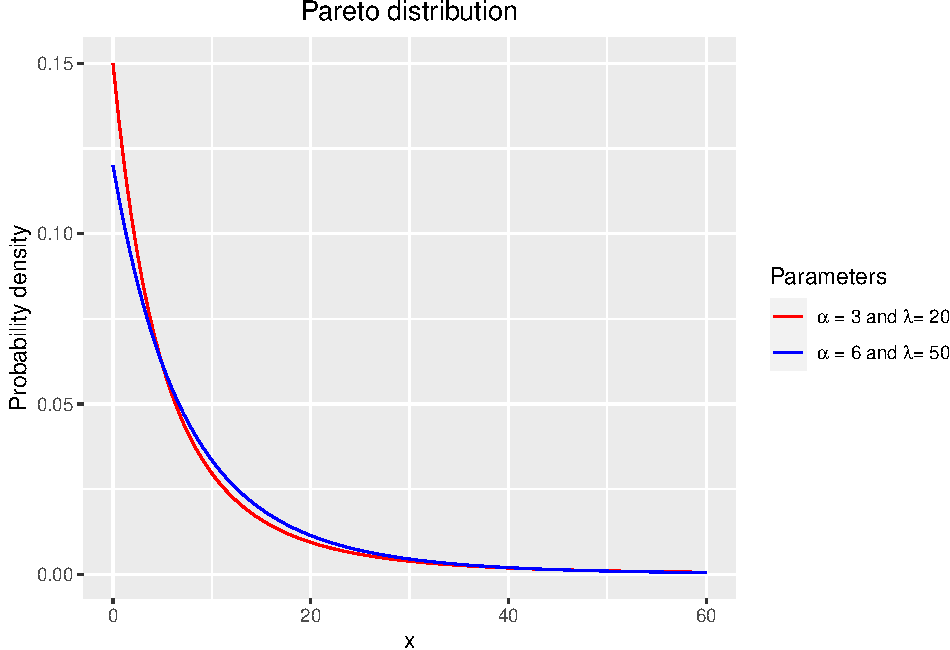
\includegraphics{SCMA470Bookdownproj_files/figure-latex/FigPareto-1.pdf}
\caption{\label{fig:FigPareto}The probability density functions (pdf) of Pareto distributions with various shape alpha and rate parameter lambda = 1.}
\end{figure}

\begin{example}
\protect\hypertarget{exm:exampleFittingClaimSizes}{}\label{exm:exampleFittingClaimSizes}

\emph{Consider a data set consisting of 200 claim amounts in
one year from a general insurance portfolio.}

\begin{enumerate}
\def\labelenumi{\arabic{enumi}.}
\item
  \emph{Calculate the sample mean and sample standard deviation.}
\item
  \emph{Use the method of moments to fit these data with both exponential
  and gamma distributions.}
\item
  \emph{Calculate the boundaries for groups or bins so that the expected
  number of claims in each bin is 20 under the fitted exponential
  distribution.}
\item
  \emph{Count the values of the observed claim amounts in each bin.}
\item
  \emph{With these bin boundaries, find the expected number of claims when
  the data are fitted with the gamma, lognormal and Pareto distributions.}
\item
  \emph{Plot a histogram for the data set along with fitted exponential
  distribution and fitted gamma distribution. In addition, plot another histogram for the data set along with fitted lognormal
  and fitted Pareto distribution.}
\item
  \emph{Comment on the goodness of fit of the fitted distributions.}
\end{enumerate}

\end{example}

\textbf{Solution:}
1. Given that \(\sum_{i=1}^n x_i = 206046.4\) and
\(\sum_{i=1}^n x_i^2 = 1,472,400,135\), we have
\[\bar{x} = \frac{\sum_{i=1}^n x_i}{n} = \frac{206046.4}{200} = 1030.232.\]
The sample variance and standard deviation are
\[s^2 = \frac{1}{n-1} \left( \sum_{i=1}^n x_i^2 - \frac{(\sum_{i=1}^n x_i)^2}{n} \right) = 6332284,\]
and \[s = 2516.403.\]

\begin{enumerate}
\def\labelenumi{\arabic{enumi}.}
\setcounter{enumi}{1}
\item
  We calculate estimates of
  unknown parameters of both exponential and gamma distributions by
  the method of moments. We simply match the mean and central moments,
  i.e.~matching \(\mathrm{E}[X]\) to the sample mean \(\bar{x}\) and
  \(\mathrm{Var}[X]\) to the sample variance.

  The MME (moment matching estimation) of the required distributions
  are as follows:

  \begin{itemize}
  \item
    the MME of \(\lambda\) for an \(\text{Exp}(\lambda)\) distribution
    is the reciprocal of the sample mean,
    \[\tilde{\lambda} = \frac{1}{\bar{x}} = 0.000971.\]
  \item
    the MMEs of \(\alpha\) and \(\lambda\) for a
    \(\mathcal{G}(\alpha, \lambda)\) distribution are
    \[\begin{aligned}
    \tilde{\alpha} &= \left(\frac{\bar{x}}{s}\right)^2 = 0.167614, \\
    \tilde{\lambda} &= \frac{\tilde{\alpha}}{\bar{x}} = 0.000163.\end{aligned}\]
  \item
    the MMEs of \(\mu\) and \(\sigma\) for a
    \(\mathcal{LN}(\mu, \sigma^2)\) distribution are \[\begin{aligned}
    \tilde{\sigma} &= \sqrt{ \ln \left(  \frac{s^2}{\bar{x}^2} + 1 \right)  }  = 1.393218, \\
    \tilde{\mu} &= \ln(\bar{x}) - \frac{\tilde{\sigma}^2 }{2} = 5.967012.\end{aligned}\]
  \item
    the MMEs of \(\alpha\) and \(\lambda\) for a
    \(\text{Pa}(\alpha, \lambda)\) distribution are \[\begin{aligned}
    \tilde{\alpha} &= \displaystyle{ 2 \left(  \frac{s^2}{\bar{x}^2} \right) \frac{1}{(\frac{s^2}{\bar{x}^2} - 1)}   } = 2.402731,\\
    \tilde{\lambda} &= \bar{x} (\tilde{\alpha} - 1) = 1445.138.\end{aligned}\]
  \end{itemize}
\item
  The upper boundaries for the 10 groups or bins so that the expected
  number of claims in each bin is 20 under the fitted exponential
  distribution are determined by
  \[\Pr(X \le \text{upbd}_j) = \frac{j}{10}, \quad j = 1,2,3, \ldots, 9.\]
  With \(\tilde{\lambda}\) from the MME for an \(\text{Exp}(\lambda)\) from the previous,
  \[\Pr(X \le x)  = 1 - \exp(-\tilde{\lambda} x).\] We obtain
  \[\text{upbd}_j = -\frac{1}{\tilde{\lambda}} \ln\left( 1 - \frac{j}{10}\right).\]
  The results are given in Table \ref{tab:tableFitted}.
\item
  The following table shows frequency distributions for observed and
  fitted claims sizes for exponential, gamma, and also lognormal and Pareto fits.
\end{enumerate}

\begin{longtable}[]{@{}rrrrrr@{}}
\caption{\label{tab:tableFitted} Frequency distributions for observed and fitted claims sizes.}\tabularnewline
\toprule
Range & Observation & Exp & Gamma & Lognormal & Pareto \\
\midrule
\endfirsthead
\toprule
Range & Observation & Exp & Gamma & Lognormal & Pareto \\
\midrule
\endhead
(0,109{]} & 60 & 20 & 109.4 & 36 & 31.9 \\
(109,230{]} & 31 & 20 & 14.3 & 34.4 & 27.8 \\
(230,367{]} & 25 & 20 & 9.7 & 26 & 24.2 \\
(367,526{]} & 17 & 20 & 7.8 & 20.5 & 21.2 \\
(526,714{]} & 14 & 20 & 6.8 & 16.6 & 18.6 \\
(714,944{]} & 13 & 20 & 6.3 & 13.9 & 16.4 \\
(944,1240{]} & 6 & 20 & 6.2 & 11.9 & 14.6 \\
(1240,1658{]} & 7 & 20 & 6.5 & 10.8 & 13.2 \\
(1658,2372{]} & 10 & 20 & 7.7 & 10.4 & 12.5 \\
(2372,\(\infty\)) & 17 & 20 & 25.4 & 19.5 & 19.4 \\
\bottomrule
\end{longtable}

\begin{enumerate}
\def\labelenumi{\arabic{enumi}.}
\setcounter{enumi}{4}
\item
  Let \(X\) be the claim size.

  \begin{itemize}
  \item
    The expected number of claims for the fitted exponential
    distribution in the range \((a,b]\) is
    \[200 \cdot \Pr( a < X \le b) = 200( e^{-\tilde{\lambda} a} - e^{-\tilde{\lambda} b} ).\]
    In our case, the expected frequencies under the fitted
    exponential distribution are given in the third column of Table \ref{tab:tableFitted}.
  \item
    (Excel) The expected number of claims for the fitted gamma distribution
    in the range \((a,b]\) is
    \[200 \cdot\left(  \text{GAMMADIST}\left(b, \tilde{\alpha}, \frac{1}{\tilde{\lambda}}, \text{TRUE}\right)  - \text{GAMMADIST}\left(a, \tilde{\alpha}, \frac{1}{\tilde{\lambda}}, \text{TRUE}\right) \right).\]
    The expected frequencies under the fitted gamma distribution are
    given in the fourth column of Table \ref{tab:tableFitted}.
  \item
    (Excel) For the fitted lognormal, the expected number of claims in the
    range \((a,b]\) can be obtained from
    \[200 \cdot\left(  \text{NORMDIST} \left(\frac{LN(b) - 
            \tilde{\mu}}{\tilde{\sigma}}\right)  - \text{NORMDIST}\left(\frac{LN(a) - 
            \tilde{\mu}}{\tilde{\sigma}}\right) \right).\]
  \item
    For the fitted Pareto distribution, the expected number of
    claims in the range \((a,b]\) can be obtained from
    \[200 \left[    \left(\frac{\tilde{\lambda}}{\tilde{\lambda} + a} \right)^{\tilde{\alpha}}  - \left(\frac{\tilde{\lambda}}{\tilde{\lambda} + b} \right)^{\tilde{\alpha}}   \right].\]
  \end{itemize}
\item
  The histograms for the data set with fitted distributions
  are shown in Figures \ref{fig:FittedExpGamma} and \ref{fig:FittedLognormalPareto}.
\item
  Comments:

  \begin{enumerate}
  \def\labelenumii{\arabic{enumii}.}
  \item
    The high positive skewness of the sample reflects the fact that
    SD is large when compared to the mean. Consequently, the
    exponential distribution may not fit the data well.
  \item
    Five claims (2.5\%) are greater than 10,000, which is one of the
    main features of the loss distribution.
  \item
    The fit is poor for the exponential distribution, as we see that
    the model under-fits the data for small claims up to 367 and
    over-fits for large claims between 944 to 2372. The gamma fit is
    again poor. We see that the model over-fits for small claims
    between 0-109 and under-fits for claims 230 and 944.
  \item
    Which one of the lognormal and Pareto distributions provides a
    better fit to the observed claim data?
  \end{enumerate}
\end{enumerate}

\begin{Shaded}
\begin{Highlighting}[]
\FunctionTok{library}\NormalTok{(stats)}
\FunctionTok{library}\NormalTok{(MASS)}
\FunctionTok{library}\NormalTok{(ggplot2)}

\NormalTok{xbar }\OtherTok{\textless{}{-}} \FunctionTok{mean}\NormalTok{(dat}\SpecialCharTok{$}\NormalTok{claims)}
\NormalTok{s }\OtherTok{\textless{}{-}} \FunctionTok{sd}\NormalTok{(dat}\SpecialCharTok{$}\NormalTok{claims)}

\CommentTok{\# MME of alpha and lambda for Gamma distribution}
\NormalTok{alpha\_tilde }\OtherTok{\textless{}{-}}\NormalTok{ (xbar}\SpecialCharTok{/}\NormalTok{s)}\SpecialCharTok{\^{}}\DecValTok{2}
\NormalTok{lambda\_tilde }\OtherTok{\textless{}{-}}\NormalTok{ alpha\_tilde}\SpecialCharTok{/}\NormalTok{xbar}

\FunctionTok{ggplot}\NormalTok{(dat) }\SpecialCharTok{+} \FunctionTok{geom\_histogram}\NormalTok{(}\FunctionTok{aes}\NormalTok{(}\AttributeTok{x =}\NormalTok{ claims, }\AttributeTok{y =}\NormalTok{ ..density..), }\AttributeTok{bins =} \DecValTok{90}\NormalTok{ , }\AttributeTok{fill =} \StringTok{"grey"}\NormalTok{, }\AttributeTok{color =} \StringTok{"black"}\NormalTok{) }\SpecialCharTok{+} 
  \FunctionTok{stat\_function}\NormalTok{(}\AttributeTok{fun=}\NormalTok{dexp, }\AttributeTok{geom =}\StringTok{"line"}\NormalTok{, }\AttributeTok{args =}\NormalTok{ (}\AttributeTok{rate =} \DecValTok{1}\SpecialCharTok{/}\FunctionTok{mean}\NormalTok{(dat}\SpecialCharTok{$}\NormalTok{claims)), }\FunctionTok{aes}\NormalTok{(}\AttributeTok{colour =} \StringTok{"Exponential"}\NormalTok{)) }\SpecialCharTok{+} 
  \FunctionTok{stat\_function}\NormalTok{(}\AttributeTok{fun=}\NormalTok{dgamma, }\AttributeTok{geom =}\StringTok{"line"}\NormalTok{, }\AttributeTok{args =} \FunctionTok{list}\NormalTok{(}\AttributeTok{shape =}\NormalTok{ alpha\_tilde ,}\AttributeTok{rate =}\NormalTok{ lambda\_tilde), }\FunctionTok{aes}\NormalTok{(}\AttributeTok{colour =} \StringTok{"Gamma"}\NormalTok{)) }\SpecialCharTok{+} \FunctionTok{ylim}\NormalTok{(}\DecValTok{0}\NormalTok{, }\FloatTok{0.0015}\NormalTok{) }\SpecialCharTok{+} \FunctionTok{scale\_color\_discrete}\NormalTok{(}\AttributeTok{name=}\StringTok{"Fitted Distributions"}\NormalTok{)}
\end{Highlighting}
\end{Shaded}

\begin{figure}
\centering
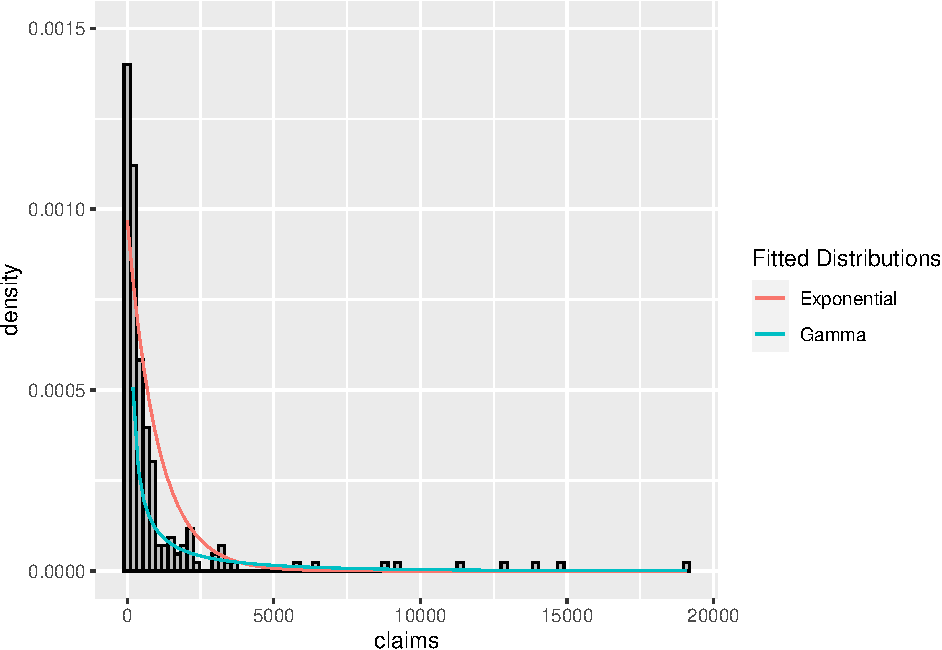
\includegraphics{SCMA470Bookdownproj_files/figure-latex/FittedExpGamma-1.pdf}
\caption{\label{fig:FittedExpGamma}Histogram of claim sizes with fitted exponential and gamma distributions.}
\end{figure}

\begin{Shaded}
\begin{Highlighting}[]
\FunctionTok{library}\NormalTok{(actuar)}
\CommentTok{\# MME of mu and sigma for lognormal distribution}

\NormalTok{sigma\_tilda }\OtherTok{\textless{}{-}} \FunctionTok{sqrt}\NormalTok{(}\FunctionTok{log}\NormalTok{(  }\FunctionTok{var}\NormalTok{(dat}\SpecialCharTok{$}\NormalTok{claims)}\SpecialCharTok{/}\FunctionTok{mean}\NormalTok{(dat}\SpecialCharTok{$}\NormalTok{claims)}\SpecialCharTok{\^{}}\DecValTok{2} \SpecialCharTok{+}\DecValTok{1}\NormalTok{  ))  }\CommentTok{\# gives \textbackslash{}tilde\textbackslash{}sigma}
\NormalTok{mu\_tilda }\OtherTok{\textless{}{-}} \FunctionTok{log}\NormalTok{(}\FunctionTok{mean}\NormalTok{(dat}\SpecialCharTok{$}\NormalTok{claims)) }\SpecialCharTok{{-}}\NormalTok{ sigma\_tilda}\SpecialCharTok{\^{}}\DecValTok{2}\SpecialCharTok{/}\DecValTok{2}      \CommentTok{\# gives \textbackslash{}tilde\textbackslash{}mu}

\CommentTok{\# MME of alpha and lambda for Pareto distribution}
\NormalTok{alpha\_tilda }\OtherTok{\textless{}{-}} \DecValTok{2}\SpecialCharTok{*}\FunctionTok{var}\NormalTok{(dat}\SpecialCharTok{$}\NormalTok{claims)}\SpecialCharTok{/}\FunctionTok{mean}\NormalTok{(dat}\SpecialCharTok{$}\NormalTok{claims)}\SpecialCharTok{\^{}}\DecValTok{2} \SpecialCharTok{*} \DecValTok{1}\SpecialCharTok{/}\NormalTok{(}\FunctionTok{var}\NormalTok{(dat}\SpecialCharTok{$}\NormalTok{claims)}\SpecialCharTok{/}\FunctionTok{mean}\NormalTok{(dat}\SpecialCharTok{$}\NormalTok{claims)}\SpecialCharTok{\^{}}\DecValTok{2} \SpecialCharTok{{-}} \DecValTok{1}\NormalTok{) }\CommentTok{\#/tilde/alpha}
\NormalTok{lambda\_tilda }\OtherTok{\textless{}{-}} \FunctionTok{mean}\NormalTok{(dat}\SpecialCharTok{$}\NormalTok{claims)}\SpecialCharTok{*}\NormalTok{(alpha\_tilda }\SpecialCharTok{{-}}\DecValTok{1}\NormalTok{)}


\FunctionTok{ggplot}\NormalTok{(dat) }\SpecialCharTok{+} \FunctionTok{geom\_histogram}\NormalTok{(}\FunctionTok{aes}\NormalTok{(}\AttributeTok{x =}\NormalTok{ claims, }\AttributeTok{y =}\NormalTok{ ..density..), }\AttributeTok{bins =} \DecValTok{90}\NormalTok{ , }\AttributeTok{fill =} \StringTok{"grey"}\NormalTok{, }\AttributeTok{color =} \StringTok{"black"}\NormalTok{) }\SpecialCharTok{+} 
  \FunctionTok{stat\_function}\NormalTok{(}\AttributeTok{fun=}\NormalTok{dlnorm, }\AttributeTok{geom =}\StringTok{"line"}\NormalTok{, }\AttributeTok{args =} \FunctionTok{list}\NormalTok{(}\AttributeTok{meanlog =}\NormalTok{ mu\_tilda, }\AttributeTok{sdlog =}\NormalTok{ sigma\_tilda), }\FunctionTok{aes}\NormalTok{(}\AttributeTok{colour =} \StringTok{"Lognormal"}\NormalTok{)) }\SpecialCharTok{+} 
  \FunctionTok{stat\_function}\NormalTok{(}\AttributeTok{fun=}\NormalTok{dpareto, }\AttributeTok{geom =}\StringTok{"line"}\NormalTok{, }\AttributeTok{args =} \FunctionTok{list}\NormalTok{(}\AttributeTok{shape =}\NormalTok{ alpha\_tilda, }\AttributeTok{scale =}\NormalTok{ lambda\_tilda), }\FunctionTok{aes}\NormalTok{(}\AttributeTok{colour =} \StringTok{"Pareto"}\NormalTok{)) }\SpecialCharTok{+}
  \FunctionTok{scale\_color\_discrete}\NormalTok{(}\AttributeTok{name=}\StringTok{"Fitted Distributions"}\NormalTok{)}
\end{Highlighting}
\end{Shaded}

\begin{figure}
\centering
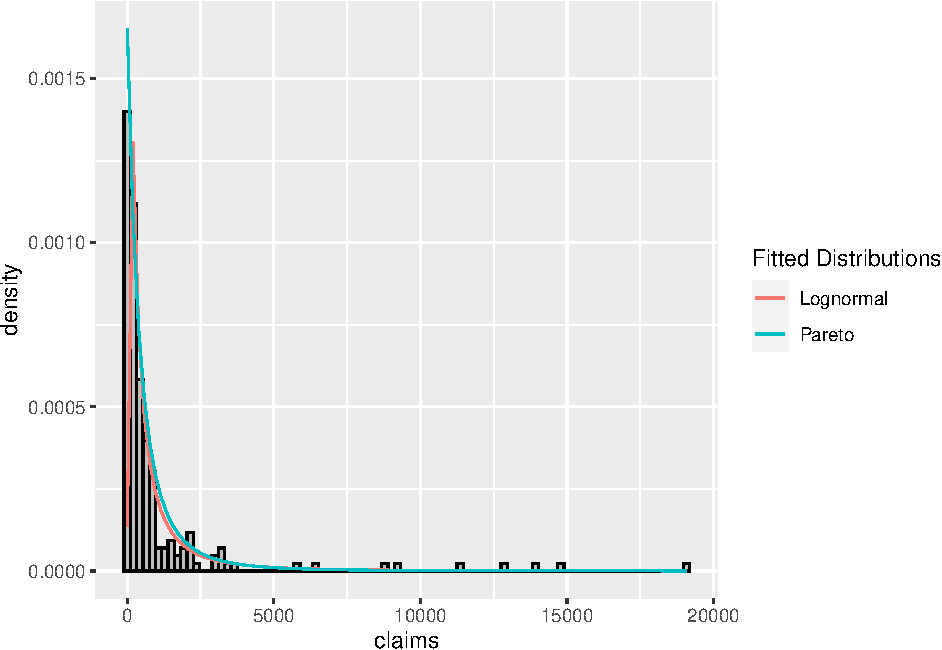
\includegraphics{SCMA470Bookdownproj_files/figure-latex/FittedLognormalPareto-1.pdf}
\caption{\label{fig:FittedLognormalPareto}Histogram of claim sizes with fitted lognormal and pareto distributions.}
\end{figure}

Let us plot the histogram of claim sizes with fitted exponential and gamma distributions in this interaction area. Note that the data set is stored in the variable \texttt{dat}.

eyJsYW5ndWFnZSI6InIiLCJwcmVfZXhlcmNpc2VfY29kZSI6ImxpYnJhcnkoc3RhdHMpXG5saWJyYXJ5KE1BU1MpXG5saWJyYXJ5KGdncGxvdDIpXG5kYXQgPC0gYygzMS4wODk0MjE1Niw5MTUuMDI1OTM2MiwzMi4wMjM3OTU2Miw4ODUuODc1NDUxLDkzMTQuMTAwNzk3LDcwNy4xNzM4ODY2LDIxMTQuMzYyNDg2LDYwMS41ODI3ODY2LDQzNS4zNzg4MTM1LDQ5LjgwMTc5NjE5LDE4MDIuMzgzODIsMjExLjYzNjQzOSwxNTMuNTk4NDcxOSw2MC4wNTk2Njk5Miw0OC4xNzE1NzY5Nyw5NDguNzIzNDYyNiwxMzIuNDI3MzEwOSwxNTEuNzEwODE1LDI5NjcuOTYxMDM2LDczNS40MTQ5MzMyLDMwNC41ODA3NTg3LDUwLjUzMzExMDY5LDIyNC43NjY1NTQ2LDM1Ni4xODA5NDM4LDQ3NS43NjY4NDQxLDMwNDQuMTQ5NTEzLDEzLjUwNjY0ODk0LDY3Ljk4Mjc0NDQ5LDMwNC4xNDM5OTY2LDIzOC4wMDAxMDUsMzk5LjA3OTgyNjMsMTQ5LjI4MDc4LDEyOC4yODQ4Mzc5LDIxLjQyMDI3NzE4LDczLjMxNDI2NzMyLDQ5LjQ2ODgyNzkxLDY2Ny41MzI3Mjc1LDQ0LjY3MzYwMTg1LDE0ODk0LjA3ODM5LDY2MC43NjE0MzA3LDEwMC43NjI4NjI4LDYzMi4yODEyMzkxLDQyLjkwODg0Nzc3LDY2LjE3NjkzMTM1LDUwLjY5NDU0MTMyLDE4Ni44NzgxNjY3LDE2OC41NDA4NjE1LDE1MS43Mzk5NzgsMjQxOS41MzIzNTQsNDM0LjQ1NjQwMzIsNjkuMDM0NjAyMzIsMTYyLjY2OTg1OTMsMjI2LjYxMTAzOTUsMzMuNjE1MDM0OTUsMjMzLjAyNzk5NiwzMjQ0Ljk0NTg5MywzNTQuMjUzNDgxMyw3OC42MTA1Mjc0NCwyMzEuNTY2NjE0LDI4My4wMjA2NDkxLDQ1Ny42Nzg1NDI2LDEzNC4yOTMzMDU4LDYxLjM0MjY1MDYzLDM4LjI1NjkxOTEyLDE1NzguOTA5MDQ4LDQ0MS42MTk5ODI2LDc2MS40MTc3Nzc3LDI3NS42OTc4NTg4LDUyMS4wMzU1OTE2LDIxODkuNjI3ODMsMTE3LjI2Njc4ODUsMjQwLjM0MDMxNTMsNjcyLjQ1MTI5MzgsNzUzLjg5NTgwMTksODQuOTg4ODMwNzksMzY2NS40MTc5NzYsNjAuMzU5Nzc1MTUsNC4wMTkzMzMwOSwxNC45NTk1MTM2NiwxOTYuNzE0NjQwMywxNTMuNzEzMzE2NSw5OC4zMTg3NTA1MywxMDQuNDQ4NjMyNCwzNTguOTIwNTg3OCwyLjI1NDk4NjMzMSwyMDU5LjYwMzk1OSwzNy42Mzg5ODYwOCw1Ni40ODk0NDAzNSwxMTQzLjA4Mjk0OCw0MTAuNzU4NTUxNiwxMi42NTQwMjk4NiwxOS44MzMyMjUxNCwxMzA1LjEzNDc5NywyMDE5LjM2MDczNSwxMjg2Ljk4NDc5LDg4OTIuMTgyMTMxLDUuODE0NTE4NzQ5LDI5Ni4xNTUxMjk1LDg2Ljc1MzA4MTYxLDQ4Ni43ODUxNDA1LDcuNDkxMzg5Nzk4LDE4MC4zMjU1MjgxLDE0MTQuMjk3NzQ4LDUyNC40NjI4MjA4LDEwNDIuNjkwMzM0LDEyOTEuNDgxNDc0LDExNS40OTUwOTk4LDM2MC42MzEwNzM3LDMyMzMuNzE2ODM4LDE0OS41MTkxMDM5LDguODQ1ODM3NDczLDgzLjg3Mjk2MzI0LDQyLjk5NjE0NTE3LDYyMy45NzA0ODUzLDQ1Ljc0OTkwMDc0LDE0NC4yNDQ5NzkzLDM2OC41NzU2NDIsODY2LjkyNzI1NDUsNTcuNjE1OTI5MjEsMTgxMi4yMzEzMTUsMjIyOS45OTg3NTQsMzQ0OC4zMzI4ODgsMTEzMTMuMzQ3MjEsMTQ5Mi40OTg4NTYsMTk2LjcyNjI1NzEsNzEuMTE4MTc2MDEsNDI1LjA2MTQ0ODMsMzguMjg2NTMwNDgsNDQuNTA5MDAxNiwzMDguODc4MTY1NywxOTA4MC41MTc0OSw4Mi4wNzYxMzkzLDI1MC4wODM1MjMsNzkuMDc0OTIwNDIsMTgzLjg2OTc2ODYsMzMuODMxNjAzOTEsMjIuNzgyMTgyOTksNjk4Ljk1NDE2NDgsMzIuNzU0MjcwMDMsNDU3LjAxMDQ5MTksMTEyLjE3MTU1NjcsMzk2LjcxNTUyMzQsMTk1LjAyNDA3ODEsMTg2My4xODUzODUsMTgxLjY0NDExMjEsNTkuMDg3MzM2NTUsOTYuMzkwMDQxOTEsODI0LjczMDE4NCwxNTUuODIxNTE2MiwxMS44NTUxMDY2MSw4NzAuODY3OTUwMiw0MjUuMzEzMzA0NSw4NTQuNzI5NjQ3NCwyNTQuMzEwODg5Miw2NjQuMzMyMDEwNyw1Ni4yNjEyMDc1MiwzNzguMjQ0MDE2LDIwNjkuNDMxNDk1LDMxMjEuMDkwMSw4NDQuNDMzNzU5NCw3NDYuMzg1MzY3NSwxODUxLjQ2OTYzMyw0MzEuNzA2MDIzMiwzMzMuMzI1NDgxLDIyLjIzOTcwMTAyLDY2Mi4zODE2ODg4LDExNy43NTkwMDU3LDU3MC40NDEyODI5LDExMjcuMDM1MzA2LDI0Ni4yNjg2MTgzLDE0NjcuNTY4ODY3LDM0Ljg5MTg3MTEyLDIzNy41NzYxNjkzLDM0OS40NTAzOTY3LDIyOS4zMzYyODQ5LDkzNC42OTI2NTYxLDE2Mi45MjU0NDA4LDU4LjI4NDk3MTcyLDEyODAzLjA0NzI2LDE1Ljk0OTA0MTg5LDk1OS45NTQzNDAyLDU4NTMuODc4OTc5LDUzNy4zOTc0MjUzLDc1LjMwNTcyODgzLDcxOC42NTk3NTIxLDYzMy44MjE0NDM4LDM2My4wMzM4MDc2LDk1Ljg0NzYyNjYsODAuMzE3ODY1MywyODYuNzEyMTc2Myw2MzY3LjQ1MzQwOCwzMjEuNTY3NzExLDIxLjUxODM4MDIyLDU5OS40NzEyOTU4LDI0Ni43MDA3MDczLDEzODYzLjc4MTgxLDIxNC43MzQyNTk3LDIzNC4zMjEyOTUyLDk1OC45MTYxNzksMTY1LjI1MjEzODUpXG5kYXQgPC0gZGF0YS5mcmFtZShjbGFpbXMgPSBkYXQpIiwic2FtcGxlIjoiIyBGaWxsIHlvdXIgY29kZSBoZXJlXG5uYW1lcyhkYXQpIiwic29sdXRpb24iOiJnZ3Bsb3QoZGF0KSArIFxuICBnZW9tX2hpc3RvZ3JhbShhZXMoeCA9IGNsYWltcywgeSA9IC4uZGVuc2l0eS4uKSwgYmlucyA9IDkwICwgZmlsbCA9IFwiZ3JleVwiLCBjb2xvciA9IFwiYmxhY2tcIikgKyBcbiAgc3RhdF9mdW5jdGlvbihmdW49ZGV4cCwgZ2VvbSA9XCJsaW5lXCIsIGFyZ3MgPSAocmF0ZSA9IDEvbWVhbihkYXQkY2xhaW1zKSksIGFlcyhjb2xvdXIgPSBcIkV4cFwiKSkgK1xuICBzY2FsZV9jb2xvcl9kaXNjcmV0ZShuYW1lPVwiRml0dGVkIERpc3RyaWJ1dGlvbnNcIikifQ==

The following code can be used to obtain the expected number of claims for the fitted exponential distribution and perform goodness-of-fit test.

eyJsYW5ndWFnZSI6InIiLCJwcmVfZXhlcmNpc2VfY29kZSI6ImxpYnJhcnkoc3RhdHMpXG5saWJyYXJ5KE1BU1MpXG5saWJyYXJ5KGdncGxvdDIpXG5kYXQgPC0gYygzMS4wODk0MjE1Niw5MTUuMDI1OTM2MiwzMi4wMjM3OTU2Miw4ODUuODc1NDUxLDkzMTQuMTAwNzk3LDcwNy4xNzM4ODY2LDIxMTQuMzYyNDg2LDYwMS41ODI3ODY2LDQzNS4zNzg4MTM1LDQ5LjgwMTc5NjE5LDE4MDIuMzgzODIsMjExLjYzNjQzOSwxNTMuNTk4NDcxOSw2MC4wNTk2Njk5Miw0OC4xNzE1NzY5Nyw5NDguNzIzNDYyNiwxMzIuNDI3MzEwOSwxNTEuNzEwODE1LDI5NjcuOTYxMDM2LDczNS40MTQ5MzMyLDMwNC41ODA3NTg3LDUwLjUzMzExMDY5LDIyNC43NjY1NTQ2LDM1Ni4xODA5NDM4LDQ3NS43NjY4NDQxLDMwNDQuMTQ5NTEzLDEzLjUwNjY0ODk0LDY3Ljk4Mjc0NDQ5LDMwNC4xNDM5OTY2LDIzOC4wMDAxMDUsMzk5LjA3OTgyNjMsMTQ5LjI4MDc4LDEyOC4yODQ4Mzc5LDIxLjQyMDI3NzE4LDczLjMxNDI2NzMyLDQ5LjQ2ODgyNzkxLDY2Ny41MzI3Mjc1LDQ0LjY3MzYwMTg1LDE0ODk0LjA3ODM5LDY2MC43NjE0MzA3LDEwMC43NjI4NjI4LDYzMi4yODEyMzkxLDQyLjkwODg0Nzc3LDY2LjE3NjkzMTM1LDUwLjY5NDU0MTMyLDE4Ni44NzgxNjY3LDE2OC41NDA4NjE1LDE1MS43Mzk5NzgsMjQxOS41MzIzNTQsNDM0LjQ1NjQwMzIsNjkuMDM0NjAyMzIsMTYyLjY2OTg1OTMsMjI2LjYxMTAzOTUsMzMuNjE1MDM0OTUsMjMzLjAyNzk5NiwzMjQ0Ljk0NTg5MywzNTQuMjUzNDgxMyw3OC42MTA1Mjc0NCwyMzEuNTY2NjE0LDI4My4wMjA2NDkxLDQ1Ny42Nzg1NDI2LDEzNC4yOTMzMDU4LDYxLjM0MjY1MDYzLDM4LjI1NjkxOTEyLDE1NzguOTA5MDQ4LDQ0MS42MTk5ODI2LDc2MS40MTc3Nzc3LDI3NS42OTc4NTg4LDUyMS4wMzU1OTE2LDIxODkuNjI3ODMsMTE3LjI2Njc4ODUsMjQwLjM0MDMxNTMsNjcyLjQ1MTI5MzgsNzUzLjg5NTgwMTksODQuOTg4ODMwNzksMzY2NS40MTc5NzYsNjAuMzU5Nzc1MTUsNC4wMTkzMzMwOSwxNC45NTk1MTM2NiwxOTYuNzE0NjQwMywxNTMuNzEzMzE2NSw5OC4zMTg3NTA1MywxMDQuNDQ4NjMyNCwzNTguOTIwNTg3OCwyLjI1NDk4NjMzMSwyMDU5LjYwMzk1OSwzNy42Mzg5ODYwOCw1Ni40ODk0NDAzNSwxMTQzLjA4Mjk0OCw0MTAuNzU4NTUxNiwxMi42NTQwMjk4NiwxOS44MzMyMjUxNCwxMzA1LjEzNDc5NywyMDE5LjM2MDczNSwxMjg2Ljk4NDc5LDg4OTIuMTgyMTMxLDUuODE0NTE4NzQ5LDI5Ni4xNTUxMjk1LDg2Ljc1MzA4MTYxLDQ4Ni43ODUxNDA1LDcuNDkxMzg5Nzk4LDE4MC4zMjU1MjgxLDE0MTQuMjk3NzQ4LDUyNC40NjI4MjA4LDEwNDIuNjkwMzM0LDEyOTEuNDgxNDc0LDExNS40OTUwOTk4LDM2MC42MzEwNzM3LDMyMzMuNzE2ODM4LDE0OS41MTkxMDM5LDguODQ1ODM3NDczLDgzLjg3Mjk2MzI0LDQyLjk5NjE0NTE3LDYyMy45NzA0ODUzLDQ1Ljc0OTkwMDc0LDE0NC4yNDQ5NzkzLDM2OC41NzU2NDIsODY2LjkyNzI1NDUsNTcuNjE1OTI5MjEsMTgxMi4yMzEzMTUsMjIyOS45OTg3NTQsMzQ0OC4zMzI4ODgsMTEzMTMuMzQ3MjEsMTQ5Mi40OTg4NTYsMTk2LjcyNjI1NzEsNzEuMTE4MTc2MDEsNDI1LjA2MTQ0ODMsMzguMjg2NTMwNDgsNDQuNTA5MDAxNiwzMDguODc4MTY1NywxOTA4MC41MTc0OSw4Mi4wNzYxMzkzLDI1MC4wODM1MjMsNzkuMDc0OTIwNDIsMTgzLjg2OTc2ODYsMzMuODMxNjAzOTEsMjIuNzgyMTgyOTksNjk4Ljk1NDE2NDgsMzIuNzU0MjcwMDMsNDU3LjAxMDQ5MTksMTEyLjE3MTU1NjcsMzk2LjcxNTUyMzQsMTk1LjAyNDA3ODEsMTg2My4xODUzODUsMTgxLjY0NDExMjEsNTkuMDg3MzM2NTUsOTYuMzkwMDQxOTEsODI0LjczMDE4NCwxNTUuODIxNTE2MiwxMS44NTUxMDY2MSw4NzAuODY3OTUwMiw0MjUuMzEzMzA0NSw4NTQuNzI5NjQ3NCwyNTQuMzEwODg5Miw2NjQuMzMyMDEwNyw1Ni4yNjEyMDc1MiwzNzguMjQ0MDE2LDIwNjkuNDMxNDk1LDMxMjEuMDkwMSw4NDQuNDMzNzU5NCw3NDYuMzg1MzY3NSwxODUxLjQ2OTYzMyw0MzEuNzA2MDIzMiwzMzMuMzI1NDgxLDIyLjIzOTcwMTAyLDY2Mi4zODE2ODg4LDExNy43NTkwMDU3LDU3MC40NDEyODI5LDExMjcuMDM1MzA2LDI0Ni4yNjg2MTgzLDE0NjcuNTY4ODY3LDM0Ljg5MTg3MTEyLDIzNy41NzYxNjkzLDM0OS40NTAzOTY3LDIyOS4zMzYyODQ5LDkzNC42OTI2NTYxLDE2Mi45MjU0NDA4LDU4LjI4NDk3MTcyLDEyODAzLjA0NzI2LDE1Ljk0OTA0MTg5LDk1OS45NTQzNDAyLDU4NTMuODc4OTc5LDUzNy4zOTc0MjUzLDc1LjMwNTcyODgzLDcxOC42NTk3NTIxLDYzMy44MjE0NDM4LDM2My4wMzM4MDc2LDk1Ljg0NzYyNjYsODAuMzE3ODY1MywyODYuNzEyMTc2Myw2MzY3LjQ1MzQwOCwzMjEuNTY3NzExLDIxLjUxODM4MDIyLDU5OS40NzEyOTU4LDI0Ni43MDA3MDczLDEzODYzLjc4MTgxLDIxNC43MzQyNTk3LDIzNC4zMjEyOTUyLDk1OC45MTYxNzksMTY1LjI1MjEzODUpXG5kYXQgPC0gZGF0YS5mcmFtZShjbGFpbXMgPSBkYXQpIiwic2FtcGxlIjoibGlicmFyeSh0aWR5cilcbmogPSAwOjlcbnVwYmQgPSBxZXhwKGovMTAsIDEvbWVhbihkYXQkY2xhaW1zKSkgICMxL21lYW4oZGF0JGNsYWltcykgZ2l2ZXMgdGhlIHBhcmFtZXRlciBvZiBleHBvbmVudGlhbCBkaXN0XG5vYnNlcnZhdGlvbiA8LSBjdXQoZGF0JGNsYWltcywgYnJlYWtzID0gdXBiZCxkaWcubGFiPTEwKVxudGFibGUob2JzZXJ2YXRpb24pXG5cbiMgVG8gZml4IHRoZSBjbGFzcyBpbnRlcnZhbCAodXBiZCB3aGVuIGogPSA5LGluZmluaXR5KVxudXBiZFtsZW5ndGgodXBiZCkrMV0gPSAxMDAwMDAwXG51cGJkXG5vYnNlcnZhdGlvbiA8LSBjdXQoZGF0JGNsYWltcywgYnJlYWtzID0gdXBiZClcblxudGFiU3VtbWFyeSA8LSB0YWJsZShvYnNlcnZhdGlvbilcblxuYmFycGxvdCh0YWJTdW1tYXJ5LG1haW49XCJDbGFpbSBzaXplc1wiLGxhcz0yKVxuXG4jIE9idGFpbiBFKEV4cCksIHRoZSBmaXR0ZWQgY2xhaW0gc2l6ZXNcbmVleHAgPC0gZGlmZigyMDAqcGV4cCh1cGJkLCByYXRlID0gMS9tZWFuKGRhdCRjbGFpbXMpKSlcblxudGFiU3VtbWFyeSA8LSBkYXRhLmZyYW1lKHRhYlN1bW1hcnkpIFxuY29sbmFtZXModGFiU3VtbWFyeSkgPC0gYyhcIlJhbmdlXCIsIFwiT2JzZXJ2YXRpb25cIilcblxudGFiU3VtbWFyeSA8LSBkYXRhLmZyYW1lKHRhYlN1bW1hcnksIEV4cG9uZW50aWFsID0gZWV4cClcblxuI3N1bW1hcnkgb2YgZXhwb25lbnRpYWwgZml0XG5jaGlzcS50ZXN0KHggPSB0YWJTdW1tYXJ5JE9ic2VydmF0aW9uLFxuICAgICAgICAgICBwID0gZWV4cC9zdW0oZWV4cCkpXG5cbiMgTWFudWFsbHkgY29tcHV0ZSBjaGktc3F1YXJlIHN0YXRpc3RpY3NcbnN1bSgodGFiU3VtbWFyeSRPYnNlcnZhdGlvbiAtIGVleHApXjIgL2VleHApICAgIn0=

\hypertarget{deductibles-and-reinsurance}{%
\chapter{Deductibles and reinsurance}\label{deductibles-and-reinsurance}}

\hypertarget{introduction-1}{%
\section{Introduction}\label{introduction-1}}

In this chapter, we will introduce the concept of risk-sharing. We will
consider two types of risk-sharing including deductibles and
reinsurance. The purpose of risk sharing is to spread the risk among the
parties involved. For example,

\begin{enumerate}
\def\labelenumi{\arabic{enumi}.}
\item
  A policyholder purchases automobile insurance with a deductible. The
  policyholder is responsible for some of the risk , and transfer the
  larger portion of the risk to the insurer. The policyholder will
  submit a claim when the loss exceeds the deductible.
\item
  A direct insurer can pass on some of the risks to another insurance
  company known as a reinsurer by purchasing insurance from the
  reinsurer. It will protect the insurer from paying large claims.
\end{enumerate}

The main goals of the chapter include the derivation of the distribution
and corresponding moments of the claim amounts paid by the policyholder,
direct insurer and the reinsurer in the presence of risk-sharing
arrangements. In addition, the effects of risk-sharing arrangements will
reduce the mean and variability of the amount paid by the direct
insurer, and also the probability that the insurer will be involved on
very large claims.

\hypertarget{deductibles}{%
\section{Deductibles}\label{deductibles}}

The insurer can modify the policy so that the policyholder is
responsible for some of the risk by including a deductible (also known
as policy excess).

Given a financial loss of \(X\) and a deductible of \(d\),

\begin{itemize}
\item
  the insured agrees to bear the first amount of \(d\) of any loss \(X\),
  and only submits a claim when \(X\) exceeds \(d\).
\item
  the insurer will pay the remaining of \(X - d\) if the loss \(X\)
  exceeds \(d\).
\end{itemize}

For example, suppose a policy has a deductible of , and you incur a loss
of in a car accident. You pay the deductible of and the car insurance
company pays the remaining of .

Let \(X\) be the claim amount, \(V\) and \(Y\) the amounts of the claim paid
by the policyholder, the (direct) insurer, respectively, i.e.
\[X = V + Y.\] So the amount paid by the policyholder and the insurer
are given by

\[\begin{aligned}
    V = 
    \begin{cases}
        X &\text{if }  X \le d\\   
        d &\text{if }  X > d,
    \end{cases} \\
    Y = 
    \begin{cases}
        0 &\text{if }  X \le d\\   
        X - d &\text{if }  X > d.
    \end{cases}\end{aligned}\] The amounts \(V\) and \(Y\) can also be
expressed as \[V = \min(X,d), \quad Y = \max(0,X-d).\]

The relationship between the policyholder and insurer is similar to that
between the insurer and reinsurer. Therefore, the detailed analysis of a
policy with a deductible is analogous to reinsurance, which will be
discussed in the following section.

\hypertarget{reinsurance}{%
\section{Reinsurance}\label{reinsurance}}

Reinsurance is insurance purchased by an insurance company in order to
protect itself from large claims. There are two main types of
reinsurance arrangement:

\begin{enumerate}
\def\labelenumi{\arabic{enumi}.}
\item
  excess of loss reinsurance; and
\item
  proportional reinsurance.
\end{enumerate}

\hypertarget{excess-of-loss-reinsurance}{%
\section{Excess of loss reinsurance}\label{excess-of-loss-reinsurance}}

Under excess of loss reinsurance arrangement, the direct insurer sets a
certain limit called a retention level \(M >0\). For a claim \(X\),

\begin{itemize}
\item
  the insurance company pays any claim in full if \(X \le M\); and
\item
  the reinsurer (or reinsurance company) pays the remaining amount of
  \(X - M\) if \(X > M\).
\end{itemize}

The position of the reinsurer under excess of loss reinsurance is the
same as that of the insurer for a policy with a deductible.

Let \(X\) be the claim amount, \(V, Y\) and \(Z\) the amounts of the claim
paid by the policyholder, (direct) insurer and reinsurer, respectively,
i.e.~\[X = V + Y + Z.\] In what follows, without stated otherwise, we
consider the case in which there is no deductible in place, i.e.~\(V = 0\)
and \[X = Y + Z.\] So the amount paid by the direct insurer and the
reinsurer are given by

\[\begin{aligned}
    Y = 
    \begin{cases}
        X &\text{if }  X \le M\\   
        M &\text{if }  X > M,
    \end{cases} \\
    Z = 
    \begin{cases}
        0 &\text{if }  X \le M\\   
        X - M &\text{if }  X > M.
    \end{cases}\end{aligned}\] The amounts \(Y\) and \(Z\) can also be
expressed as \[Y = \min(X,M), \quad Z = \max(0,X-M).\]

d = 1000 M = 10000 X = \[3000, 800, 25000, 5000, 20000\]

\begin{example}
\protect\hypertarget{exm:examplePayouts}{}\label{exm:examplePayouts}

Suppose a policy has a deductible of and the
insurer arrange excess of loss reinsurance with retention level of . A
sample of loss amounts in one year consists of the following values, in
unit of Thai baht: \[3000, 800, 25000, 5000, 20000 .\] Calculate the
total amount paid by:*

\begin{enumerate}
\def\labelenumi{\arabic{enumi}.}
\item
  \emph{the policyholder;}
\item
  \emph{the insurer; and}
\item
  \emph{the reinsurer.}
\end{enumerate}

\end{example}

\textbf{Solution:}

The total amounts paid by

\begin{itemize}
\item
  the policyholders : \[1000 + 800 + 1000 + 1000 + 1000 = 4800.\]
\item
  The insurer : \[2000 + 0 + 10000 + 4000 + 10000 = 26000.\]
\item
  The reinsurer : \[0 + 0 + 14000 + 0 + 9000 = 23000.\]
\end{itemize}

\hypertarget{mixed-distributions}{%
\section{Mixed distributions}\label{mixed-distributions}}

In the subsequent sections, we will derive the probability distribution
of the random variables \(Y\) and \(Z\), which are the insurer's and
reinsurer's payouts on claims. Their distributions are neither purely
continuous, nor purely discrete. First we start with some important
properties of such random variables.

A random variable \(U\) which is partly discrete and partly continuous is
said to be a mixed distribution. The distribution function of \(U\),
denoted by \(F_U(x)\) is continuous and differentiable except for some
values of \(x\) in a countable set \(S\). For a mixed distribution \(U\),
there exists a function \(f_U(x)\) such that
\[F_U(x) = \Pr(U \le x) = \int_{-\infty}^x f_U(x) dx + \sum_{x_i \in S, x_i \le x } \Pr(U = x_i).\]
The expected value of \(g(U)\) for some function \(g\) is given by

\begin{equation} 
\label{eq:eqnExpectationMixed} \mathrm{E}[g(U)] = \int_{-\infty}^\infty g(x) f_U(x) \mathop{}\!d{x} + \sum_{x_i \in S } g(x_i) \Pr(U = x_i).
\end{equation}

It is the sum of the integral over the intervals at which \(f_U(x)\) is
continuous and the summation over the points in \(S\).

The function \(f_U(x)\) is not the probability density function of \(U\)
because \(\int_{-\infty}^\infty f_U(x) dx \neq 1\). In particular, it is
the derivative of \(F_U(x)\) at the points where \(F_U(x)\) is continuous
and differentiable.

Recall that \(X\) denotes the claim amount and \(Y\) and \(Z\) be the amounts
of the claim paid by the insurer and reinsurer. The distribution
function and the density function of the claim amount \(X\) are denoted by
\(F_{X}\) and \(f_X(x)\), where we assume that \(X\) is continuous. In the
following examples, we will derive the distribution, mean and variance
of the random variables \(Y\) and \(Z\). Furthermore, both random variables
\(Y\) and \(Z\) are examples of mixed distributions.

\begin{example}
\protect\hypertarget{exm:unlabeled-div-30}{}\label{exm:unlabeled-div-30}

\emph{Let \(F_Y\) denote the distribution function of
\(Y = \min(X,M)\). It follows that \[F_Y(x) = 
    \begin{cases}
        F_X(x) &\text{if }  x < M\\   
        1 &\text{if }  x \ge M
    \end{cases}.\] Hence, the distribution function of \(Y\) is said to be
a mixed distribution.}

\end{example}

\textbf{Solution:}
From \(Y = \min(X,M)\), if \(y < M\), then
\[F_Y(y) = \Pr(Y \le y) = \Pr(X \le y) = F_X(y).\] If \(y \ge M\), then
\[F_Y(y) = \Pr(Y \le y) = 1,\] which follows because \(\min(X,M) \le M\).

Hence, \(Y\) is mixed with a density function \(f_X(x)\), for \(0 \le x < M\)
and a mass of probability at \(M\), with \(Pr(Y = M) = 1 - F_X(M)\). The
last equality follows from \[\begin{aligned}
    \Pr(Y = M) &= \Pr(X > M) \\
        &=   1 - \Pr(X \le M) = 1 - F_X(M). \end{aligned}\]

\begin{example}
\protect\hypertarget{exm:unlabeled-div-31}{}\label{exm:unlabeled-div-31}

\emph{Show that
\[\mathrm{E}[Y] = \mathrm{E}[\min(X,M)] = \mathrm{E}[X] - \int_0^\infty y f_X(y+M) \mathop{}\!dy.\]}

\end{example}

\(\mathrm{E}[Y]\) is the expected payout by the insurer.

\[\begin{aligned}
    \mathrm{E}[Y] &= \mathrm{E}[\min(X,M)] \\
        &= \int_0^\infty \min(X,M) \cdot f_X(x) \, dx \\
        &= \int_0^M x \cdot f_X(x) \, dx + \int_M^\infty M \cdot f_X(x) \, dx \\
        &= \int_0^M x \cdot f_X(x) \, dx + \int_M^\infty x \cdot f_X(x) \, dx + \int_M^\infty (M - x) \cdot f_X(x) \, dx \\
        &= \mathrm{E}[X] + \int_M^\infty (M - x) \cdot f_X(x) \, dx \\
    &= \mathrm{E}[X] + \int_0^\infty (-y) \cdot f_X(y+M) \, dy \\
    &=  \mathrm{E}[X] - \int_0^\infty y \cdot f_X(y+M) \, dy 
\end{aligned}\]

\textbf{Note}
Under excess of loss reinsurance arrangement, the mean amount paid by
the insurer is reduced by the amount equal to
\(\int_0^\infty y f_X(y+M) \mathop{}\!dy.\)

\begin{example}
\protect\hypertarget{exm:unlabeled-div-32}{}\label{exm:unlabeled-div-32}

\emph{Let \(X\) be an exponential distribution with parameter
\(\lambda\) and \(Y = \min(X,M)\). Then \[F_Y(x) = 
    \begin{cases}
        1 - e^{-\lambda x} &\text{if }  x < M\\   
        1 &\text{if }  x \ge M
    \end{cases}.\] A plot of the distribution function \(F_Y\) is given in
Figure~\protect\hyperlink{figMixedDist}{1}. Hence, \(Y\) is a mixed distribution with a
density function \(f_Y(x) = f_X(x)\) for \(0 < x < M\) and a probability
mass at \(M\) is \(\Pr(Y = M) = 1 - F_X(M)\).}

Using
\eqref{eq:eqnExpectationMixed}, the expected value of \(Y\),
\(\mathrm{E}[Y]\) is given by

\[\begin{aligned}
    \mathrm{E}[Y] &= \int_{0}^M x f_X(x) \mathop{}\!d{x}  + M(1 - F_X(M)).  \end{aligned}\]

\end{example}

\begin{example}
\protect\hypertarget{exm:unlabeled-div-33}{}\label{exm:unlabeled-div-33}

\emph{Let \(F_Z\) denote the distribution function of
\(Z = \max(0,X-M)\). It follows that \[F_Z(x) = 
    \begin{cases}
        F_{X}(M) &\text{if }  x = 0\\   
        F_{X}(x + M) &\text{if }  x > 0
    \end{cases}.\] Hence, the distribution function of \(Z\) is a mixed
distribution with a mass of probability at \(0\).}

\end{example}

\textbf{Solution:}
The random variable \(Z\) is the \textbf{reinsurer's payout} which also include
\textbf{zero claims}. Later we will consider only \textbf{reinsurance claims},
which involve the reinsurer, i.e.~claims such that \(X > M\).

The distribution of \(Z\) can be derived as follows:

\begin{itemize}
\item
  For \(x =0\), \[F_Z(0) = \Pr(Z = 0) = \Pr(X \le M) = F_X(M).\]
\item
  For \(x > 0\), \[\begin{aligned}
      F_Z(0) &= \Pr(Z \le x) = \Pr(\max(0,X-M) \le x) \\
      &= \Pr(X- M \le x) = \Pr(X \le x + M) = F_X(x + M).\end{aligned}\]
\end{itemize}

\begin{example}
\protect\hypertarget{exm:unlabeled-div-34}{}\label{exm:unlabeled-div-34}

\emph{Let \(X\) be an exponential distribution with parameter
\(\lambda\) and \(Z = \max(0,X-M)\). Derive and plot the probability
distribution \(F_Z\) for \(\lambda = 1\) and \(M = 2\).}

\end{example}

\begin{example}
\protect\hypertarget{exm:unlabeled-div-35}{}\label{exm:unlabeled-div-35}

\emph{Show that
\[\mathrm{E}[Z] = \mathrm{E}[\max(0,X-M)] = \int_M^\infty (x- M) f_X(x) \mathop{}\!dx = \int_0^\infty y f_X(y+M) \mathop{}\!dy.\]
Comment on the result.}

\end{example}

\textbf{Solution:}
The expected payout on the claim by the reinsurer, \(\mathrm{E}[Z]\), and
can also be found directly as follows: \[\begin{aligned}
\mathrm{E}[Z] &= \mathrm{E}[\max(0,X-M)] \\
    &= \int_0^M 0 \cdot f_X(x) \, dx + \int_M^\infty (X-M) \cdot f_X(x) \, dx \\
    &= 0 +  \int_0^\infty y \cdot f_X(y + M) \, dy.\end{aligned}\] It
follows from the previous results that
\[\mathrm{E}[X] = \mathrm{E}[Y + Z] =  \mathrm{E}[Y]+ \mathrm{E}[Z].\]

\begin{example}
\protect\hypertarget{exm:unlabeled-div-36}{}\label{exm:unlabeled-div-36}

\emph{Let the claim amount \(X\) have exponential distribution
with mean \(\mu = 1/\lambda\).}

\begin{enumerate}
\def\labelenumi{\arabic{enumi}.}
\item
  \emph{Find the proportion of claims which involve the reinsurer.}
\item
  \emph{Find the insurer's expected payout on a claim.}
\item
  \emph{Find the reinsurer's expected payout on a claim.}
\end{enumerate}

\end{example}

\textbf{Solution:}
1. The proportion of claims which involve the reinsurer is
\[\Pr(X > M) = 1 - F_X(M) = e^{-\lambda M} = e^{-M/\mu}.\]

\begin{enumerate}
\def\labelenumi{\arabic{enumi}.}
\setcounter{enumi}{1}
\item
  The insurer's expected payout on a claim can be calculated by
  \[\begin{aligned}
      \mathrm{E}[Y] &= \mathrm{E}[X] -  \int_0^\infty y \cdot \lambda e^{-\lambda(y+M)} \, dy \\
          &= \mathrm{E}[X] - e^{-\lambda M} \int_0^\infty y \cdot \lambda e^{-\lambda \cdot y} \, dy \\
          &= \mathrm{E}[X] - e^{-\lambda M}  \mathrm{E}[X] \\
          &= (1 - e^{-\lambda M})  \mathrm{E}[X].\end{aligned}\]
\item
  It follows from the above result that the reinsurer's expected
  payout on a claim is \(e^{-\lambda M} \mathrm{E}[X].\)
\end{enumerate}

\begin{example}
\protect\hypertarget{exm:unlabeled-div-37}{}\label{exm:unlabeled-div-37}

\emph{An insurer covers an individual loss \(X\) with excess of
loss reinsurance with retention level \(M\). Let \(f_X(x)\) and \(F_X(x)\)
denote the pdf and cdf of \(X\), respectively.}

\begin{enumerate}
\def\labelenumi{\arabic{enumi}.}
\item
  \emph{Show that the variance of the amount paid by the insurer on a
  single claim satisfies:
  \[\mathrm{Var}[\min(X,M)] = \int_0^M x^2 f_X(x) \mathop{}\!dx + M^2 (1 - F_X(M)) - (\mathrm{E}[\min(X,M)])^2.\]}
\item
  \emph{Show that the variance of the amount paid by the reinsurer on a
  single claim satisfies:
  \[\mathrm{Var}[\max(0,X-M)] = \int_M^\infty (x-M)^2 f_X(x) \mathop{}\!dx  - (\mathrm{E}[\max(0,X-M)])^2.\]}
\end{enumerate}

\end{example}

\hypertarget{the-distribution-of-reinsurance-claims}{%
\section{The distribution of reinsurance claims}\label{the-distribution-of-reinsurance-claims}}

In practice, the reinsurer involves only claims which exceed the
retention limit, i.e.~\(X > M\). Information of claims which are less or
equal to \(M\) may not be available to the reinsurer. The claim amount \(Z\)
paid by the reinsurer can be modified accordingly to take into account
of non-zero claim sizes.

Recall from
Example \ref{exm:examplePayouts}, there are only three claims whose amounts
exceed the retention level of . Such claims, consisting of , 9000 and
23000 which involves the reinsurer are known as \textbf{reinsurance claims}.

Let \(W = Z|Z>0\) be a random variable representing the amount of a
non-zero payment by the reinsurer on a reinsurance claim. The
distribution and density of \(W\) can be calculated as follows: for
\(x > 0\), \[\begin{aligned}
     \Pr[W \le x ] &= \Pr[Z \le x | Z >0] \\
            &= \Pr[X - M \le x | X > M] \\
            &= \frac{\Pr[M < X \le x + M]}{\Pr[X > M]}\\
            &= \frac{F_X(x+M) - F_X(M)}{1-F_X(M)}.\end{aligned}\]
Differentiating with respect to \(x\), we obtain the density function of
\(W\) as \[f_W(x) = \frac{f_X(x+M)}{1 - F_X(M)}.\] Hence, the mean and
variance can be directly obtained from the density function of \(W\).

\hypertarget{proportional-reinsurance}{%
\section{Proportional reinsurance}\label{proportional-reinsurance}}

Under excess of loss reinsurance arrangement, the direct insurer pays a
fixed proportion \(\alpha\), called the proportion of the risk retained by
the insurer, and the reinsurer pays the remainder of the claim.

Let \(X\) be the claim amount, \(Y\) and \(Z\) the amounts of the claim paid
by the policyholder, (direct) insurer and reinsurer, respectively, i.e.
\[X = Y + Z.\] So the amount paid by the direct insurer and the
reinsurer are given by \[Y = \alpha X, \quad Z = (1 - \alpha) X.\] Both
of the random variables are scaled by the factor of \(\alpha\) and
\(1- \alpha\), respectively.

\begin{example}
\protect\hypertarget{exm:unlabeled-div-38}{}\label{exm:unlabeled-div-38}

\emph{Derive the distribution function and density function
of \(Y\).}

\end{example}

\textbf{Solution:}
Let \(X\) has a distribution function \(F\) with density function \(f\). The
distribution function of \(Y\) is given by \[\Pr(Y \le x) = F(x/a).\]
Hence, the density function is \[f_Y(x) = \frac{1}{a}f(x/a).\]

You can get more examples from Tutorials.

\hypertarget{tutorials}{%
\chapter{Tutorials}\label{tutorials}}

\hypertarget{tutorial-1}{%
\section{Tutorial 1}\label{tutorial-1}}

\begin{enumerate}
\def\labelenumi{\arabic{enumi}.}
\item
  Using the method of moments, calculate the parameter values for the
  gamma, lognormal and Pareto distributions for which
  \[\mathrm{E}[X] = 500 \quad  \text{and} \quad  \mathrm{Var}[X] = 100^2.\]
\item
  Show that if \(X \sim \text{Exp}(\lambda)\), then the random variable
  \(X-w\) conditional on \(X > w\) has the same distribution as \(X\), i.e.
  \[X \sim \text{Exp}(\lambda)\Rightarrow  X - w | X > w \sim \text{Exp}(\lambda).\]
\item
  Derive an expression for the variance of the
  \(\text{Pa}(\alpha, \lambda)\) distribution. (Hint: using the pdf)
\item
  Show that the MLE (the maximum likelihood estimation) of \(\lambda\)
  for an \(\text{Exp}(\lambda)\) distribution is the reciprocal of the
  sample mean, i.e.~\(\hat\lambda = 1/ \bar x\).
\item
  Claims last year on a portfolio of policies of a risk had a
  lognormal distribution with parameter \(\mu = 5\) and
  \(\sigma^2 = 0.4\). It is estimated that all claims will increase by
  15\% next year. Find the probability that a claim next year will
  exceed 1000.
\end{enumerate}

\hypertarget{tutorial-2}{%
\section{Tutorial 2}\label{tutorial-2}}

\begin{enumerate}
\def\labelenumi{\arabic{enumi}.}
\item
  Claims occur on a general insurance portfolio independently and at
  random. Each claim is classified as being of ``Type A'' or ``Type B''.
  Type A claim amounts are distributed \(\text{Pa}(3,400)\) and Type B
  claim amounts are distributed \(\text{Pa}(4,1000)\). It is known that
  90\% of all claims are of Type A.

  Let \(X\) denote a claim chosen at random from the portfolio.

  \begin{enumerate}
  \def\labelenumii{\arabic{enumii}.}
  \item
    Calculate \(\Pr(X > 1000).\)
  \item
    Calculate \(\mathrm{E}[X]\) and \(\mathrm{Var}[X]\).
  \item
    Let \(Y\) have a Pareto distribution
    with the same mean and variance as \(X\). Calculate
    \(\Pr(Y > 1000).\)
  \item
    Comment on the difference in the answers found in 1.1 and 1.2.
  \end{enumerate}
\item
  An insurer covers an individual loss \(X\) with excess of loss
  reinsurance with retention level \(M\). Let \(Y\) and \(Z\) be random
  variables representing the amounts paid by the insurer and
  reinsurer, respectively, i.e.~\(X = Y + Z\). Show that
  \(\mathrm{Cov}[Y,Z] \ge 0\) and deduce that
  \[\mathrm{Var}[X] \ge \mathrm{Var}[Y] +  \mathrm{Var}[Z].\] Comment
  on the results obtained.
\item
  Claim amounts from a general insurance portfolio are lognormally
  distributed with mean 200 and variance 2916. Excess of loss
  reinsurance with retenton level 250 is arranged. Calculate the
  probability that the reinsurer is involved in a claim.
\item
  Show that if \(X \sim \text{Pa}(\alpha, \lambda)\), then the random
  variable \(X-d\) conditional on \(X > d\) has a pareto distribution with
  parameters \(\alpha\) and \(\lambda + d\), i.e.
  \[X \sim \text{Pa}(\alpha, \lambda)\Rightarrow  X - d | X > d \sim \text{Pa}(\alpha,\lambda + d).\]
\item
  Consider a portfolio of motor insurance policies. In the event of an
  accident, the cost of the repairs to a car has a Pareto distribution
  with parameters \(\alpha\) and \(\lambda\). A deductible of 100 is
  applied to all claims and a claim is always made if the cost of the
  repairs exceeds this amount. A sample of 100 claims has mean 200 and
  standard deviation 250.

  \begin{enumerate}
  \def\labelenumii{\arabic{enumii}.}
  \item
    Using the method of moments, estimate \(\alpha\) and \(\lambda\).
  \item
    Estimate the proportion of accidents that do not result in a
    claim being made.
  \item
    The insurance company arranges excess of loss reinsurance with
    another insurance company to reduce the mean amount it pays on a
    claim to 160. Calculate the retention limit needed to achieve
    this.
  \end{enumerate}
\end{enumerate}

\hypertarget{interactive-lecture}{%
\chapter{Interactive Lecture}\label{interactive-lecture}}

Some \emph{significant} applications are demonstrated in this chapter.

\hypertarget{datacamp-light}{%
\section{DataCamp Light}\label{datacamp-light}}

By default, \texttt{tutorial} will convert all R chunks.

eyJsYW5ndWFnZSI6InIiLCJzYW1wbGUiOiJhIDwtIDJcbmIgPC0gM1xuYSArIGIifQ==

eyJsYW5ndWFnZSI6InIiLCJwcmVfZXhlcmNpc2VfY29kZSI6ImxpYnJhcnkoc3RhdHMpXG5saWJyYXJ5KE1BU1MpXG5saWJyYXJ5KGdncGxvdDIpXG5kYXQgPC0gYygzMS4wODk0MjE1Niw5MTUuMDI1OTM2MiwzMi4wMjM3OTU2Miw4ODUuODc1NDUxLDkzMTQuMTAwNzk3LDcwNy4xNzM4ODY2LDIxMTQuMzYyNDg2LDYwMS41ODI3ODY2LDQzNS4zNzg4MTM1LDQ5LjgwMTc5NjE5LDE4MDIuMzgzODIsMjExLjYzNjQzOSwxNTMuNTk4NDcxOSw2MC4wNTk2Njk5Miw0OC4xNzE1NzY5Nyw5NDguNzIzNDYyNiwxMzIuNDI3MzEwOSwxNTEuNzEwODE1LDI5NjcuOTYxMDM2LDczNS40MTQ5MzMyLDMwNC41ODA3NTg3LDUwLjUzMzExMDY5LDIyNC43NjY1NTQ2LDM1Ni4xODA5NDM4LDQ3NS43NjY4NDQxLDMwNDQuMTQ5NTEzLDEzLjUwNjY0ODk0LDY3Ljk4Mjc0NDQ5LDMwNC4xNDM5OTY2LDIzOC4wMDAxMDUsMzk5LjA3OTgyNjMsMTQ5LjI4MDc4LDEyOC4yODQ4Mzc5LDIxLjQyMDI3NzE4LDczLjMxNDI2NzMyLDQ5LjQ2ODgyNzkxLDY2Ny41MzI3Mjc1LDQ0LjY3MzYwMTg1LDE0ODk0LjA3ODM5LDY2MC43NjE0MzA3LDEwMC43NjI4NjI4LDYzMi4yODEyMzkxLDQyLjkwODg0Nzc3LDY2LjE3NjkzMTM1LDUwLjY5NDU0MTMyLDE4Ni44NzgxNjY3LDE2OC41NDA4NjE1LDE1MS43Mzk5NzgsMjQxOS41MzIzNTQsNDM0LjQ1NjQwMzIsNjkuMDM0NjAyMzIsMTYyLjY2OTg1OTMsMjI2LjYxMTAzOTUsMzMuNjE1MDM0OTUsMjMzLjAyNzk5NiwzMjQ0Ljk0NTg5MywzNTQuMjUzNDgxMyw3OC42MTA1Mjc0NCwyMzEuNTY2NjE0LDI4My4wMjA2NDkxLDQ1Ny42Nzg1NDI2LDEzNC4yOTMzMDU4LDYxLjM0MjY1MDYzLDM4LjI1NjkxOTEyLDE1NzguOTA5MDQ4LDQ0MS42MTk5ODI2LDc2MS40MTc3Nzc3LDI3NS42OTc4NTg4LDUyMS4wMzU1OTE2LDIxODkuNjI3ODMsMTE3LjI2Njc4ODUsMjQwLjM0MDMxNTMsNjcyLjQ1MTI5MzgsNzUzLjg5NTgwMTksODQuOTg4ODMwNzksMzY2NS40MTc5NzYsNjAuMzU5Nzc1MTUsNC4wMTkzMzMwOSwxNC45NTk1MTM2NiwxOTYuNzE0NjQwMywxNTMuNzEzMzE2NSw5OC4zMTg3NTA1MywxMDQuNDQ4NjMyNCwzNTguOTIwNTg3OCwyLjI1NDk4NjMzMSwyMDU5LjYwMzk1OSwzNy42Mzg5ODYwOCw1Ni40ODk0NDAzNSwxMTQzLjA4Mjk0OCw0MTAuNzU4NTUxNiwxMi42NTQwMjk4NiwxOS44MzMyMjUxNCwxMzA1LjEzNDc5NywyMDE5LjM2MDczNSwxMjg2Ljk4NDc5LDg4OTIuMTgyMTMxLDUuODE0NTE4NzQ5LDI5Ni4xNTUxMjk1LDg2Ljc1MzA4MTYxLDQ4Ni43ODUxNDA1LDcuNDkxMzg5Nzk4LDE4MC4zMjU1MjgxLDE0MTQuMjk3NzQ4LDUyNC40NjI4MjA4LDEwNDIuNjkwMzM0LDEyOTEuNDgxNDc0LDExNS40OTUwOTk4LDM2MC42MzEwNzM3LDMyMzMuNzE2ODM4LDE0OS41MTkxMDM5LDguODQ1ODM3NDczLDgzLjg3Mjk2MzI0LDQyLjk5NjE0NTE3LDYyMy45NzA0ODUzLDQ1Ljc0OTkwMDc0LDE0NC4yNDQ5NzkzLDM2OC41NzU2NDIsODY2LjkyNzI1NDUsNTcuNjE1OTI5MjEsMTgxMi4yMzEzMTUsMjIyOS45OTg3NTQsMzQ0OC4zMzI4ODgsMTEzMTMuMzQ3MjEsMTQ5Mi40OTg4NTYsMTk2LjcyNjI1NzEsNzEuMTE4MTc2MDEsNDI1LjA2MTQ0ODMsMzguMjg2NTMwNDgsNDQuNTA5MDAxNiwzMDguODc4MTY1NywxOTA4MC41MTc0OSw4Mi4wNzYxMzkzLDI1MC4wODM1MjMsNzkuMDc0OTIwNDIsMTgzLjg2OTc2ODYsMzMuODMxNjAzOTEsMjIuNzgyMTgyOTksNjk4Ljk1NDE2NDgsMzIuNzU0MjcwMDMsNDU3LjAxMDQ5MTksMTEyLjE3MTU1NjcsMzk2LjcxNTUyMzQsMTk1LjAyNDA3ODEsMTg2My4xODUzODUsMTgxLjY0NDExMjEsNTkuMDg3MzM2NTUsOTYuMzkwMDQxOTEsODI0LjczMDE4NCwxNTUuODIxNTE2MiwxMS44NTUxMDY2MSw4NzAuODY3OTUwMiw0MjUuMzEzMzA0NSw4NTQuNzI5NjQ3NCwyNTQuMzEwODg5Miw2NjQuMzMyMDEwNyw1Ni4yNjEyMDc1MiwzNzguMjQ0MDE2LDIwNjkuNDMxNDk1LDMxMjEuMDkwMSw4NDQuNDMzNzU5NCw3NDYuMzg1MzY3NSwxODUxLjQ2OTYzMyw0MzEuNzA2MDIzMiwzMzMuMzI1NDgxLDIyLjIzOTcwMTAyLDY2Mi4zODE2ODg4LDExNy43NTkwMDU3LDU3MC40NDEyODI5LDExMjcuMDM1MzA2LDI0Ni4yNjg2MTgzLDE0NjcuNTY4ODY3LDM0Ljg5MTg3MTEyLDIzNy41NzYxNjkzLDM0OS40NTAzOTY3LDIyOS4zMzYyODQ5LDkzNC42OTI2NTYxLDE2Mi45MjU0NDA4LDU4LjI4NDk3MTcyLDEyODAzLjA0NzI2LDE1Ljk0OTA0MTg5LDk1OS45NTQzNDAyLDU4NTMuODc4OTc5LDUzNy4zOTc0MjUzLDc1LjMwNTcyODgzLDcxOC42NTk3NTIxLDYzMy44MjE0NDM4LDM2My4wMzM4MDc2LDk1Ljg0NzYyNjYsODAuMzE3ODY1MywyODYuNzEyMTc2Myw2MzY3LjQ1MzQwOCwzMjEuNTY3NzExLDIxLjUxODM4MDIyLDU5OS40NzEyOTU4LDI0Ni43MDA3MDczLDEzODYzLjc4MTgxLDIxNC43MzQyNTk3LDIzNC4zMjEyOTUyLDk1OC45MTYxNzksMTY1LjI1MjEzODUpXG5kYXQgPC0gZGF0YS5mcmFtZShjbGFpbXMgPSBkYXQpIiwic2FtcGxlIjoiIyBGaWxsIHlvdXIgY29kZSBoZXJlXG5uYW1lcyhkYXQpIiwic29sdXRpb24iOiJnZ3Bsb3QoZGF0KSArIFxuICBnZW9tX2hpc3RvZ3JhbShhZXMoeCA9IGNsYWltcywgeSA9IC4uZGVuc2l0eS4uKSwgYmlucyA9IDkwICwgZmlsbCA9IFwiZ3JleVwiLCBjb2xvciA9IFwiYmxhY2tcIikgKyBcbiAgc3RhdF9mdW5jdGlvbihmdW49ZGV4cCwgZ2VvbSA9XCJsaW5lXCIsIGFyZ3MgPSAocmF0ZSA9IDEvbWVhbihkYXQkY2xhaW1zKSksIGFlcyhjb2xvdXIgPSBcIkV4cFwiKSkgK1xuICBzY2FsZV9jb2xvcl9kaXNjcmV0ZShuYW1lPVwiRml0dGVkIERpc3RyaWJ1dGlvbnNcIikifQ==

  \bibliography{book.bib,packages.bib}

\end{document}
